\documentclass{overturerepchap}
%**********************************************************
%
% Bibliography support
%
%**********************************************************
%\def\@reportno{YY--NN}		% default report no.
%\def\reportno#1{\gdef\@reportno{#1}}
\usepackage{fancyhdr}
\usepackage{longtable}
\newcommand{\bthisbibliography}[1]{\chapter*{References}%
   \begin {list} {}%
     {\settowidth {\labelwidth} {[#1]XX}%
      \setlength {\leftmargin} {\labelwidth}%
      \addtolength{\leftmargin} {\labelsep}%
      \setlength {\parsep} {1ex}%
      \setlength {\itemsep} {2ex}%
     }
  }
\newcommand{\ethisbibliography}{\end{list}}
\newcommand{\refitem}[2]
  {\bibitem[#1]{#2}}

\newcommand{\back}{$\setminus$}
\newcommand{\RuleTarget}[1]{\hypertarget{rule:#1}{}}
\newcommand{\Ruledef}[2]
{
  \RuleTarget{#1}\Rule{#1}{#2}%
  }
\newcommand{\Ruleref}[1]{
  \hyperlink{rule:#1}{#1}}
\newcommand{\Lit}[1]{`{\tt #1}\Quote}
\newcommand{\Rule}[2]{
  \begin{quote}\begin{tabbing}
    #1\index{#1}\ \ \= = \ \ \= #2  ; %    Adds production rule to index
    
  \end{tabbing}\end{quote}
  }
\newcommand{\SeqPt}[1]{\{\ #1\ \}}
\newcommand{\lfeed}{\\ \> \>}
\newcommand{\dsepl}{\ $|$\ }
\newcommand{\dsep}{\\ \> $|$ \>}
\newcommand{\Lop}[1]{`{\sf #1}\Quote}
\newcommand{\blankline}{\vspace{\baselineskip}}
\newcommand{\Brack}[1]{(\ #1\ )}
\newcommand{\nmk}{\footnotemark}
\newcommand{\ntext}[1]{\footnotetext{{\bf Note: } #1}}
\newlength{\kwlen}
\newcommand{\Keyw}[1]{\settowidth{\kwlen}{\tt #1}\makebox[\kwlen][l]{\sf
    #1}}
\newcommand{\keyw}[1]{{\sf #1}}
\newcommand{\id}[1]{{\tt #1}}
\newcommand{\metaiv}[1]{\begin{alltt}\input{#1}\end{alltt}}

\newcommand{\OptPt}[1]{[\ #1\ ]}
\newcommand{\MAP}[2]{\kw{map }#1\kw{ to }#2}
\newcommand{\INMAP}[2]{\kw{inmap }#1\kw{ to }#2}
\newcommand{\SEQ}[1]{\kw{seq of }#1}
\newcommand{\NSEQ}[1]{\kw{seq1 of }#1}
\newcommand{\SET}[1]{\kw{set of }#1}
\newcommand{\PROD}[2]{#1 * #2}
\newcommand{\TO}[2]{$#1 \To #2$}
\newcommand{\FUN}[2]{#1 \To #2}
\newcommand{\PUBLIC}{\ifthenelse{\boolean{VDMpp}}{public\mbox{}}{\mbox{}}}
\newcommand{\PRIVATE}{\ifthenelse{\boolean{VDMpp}}{private}{\mbox{}}}
\newcommand{\PROTECTED}{\ifthenelse{\boolean{VDMpp}}{protected}{\mbox{}}}

\pagestyle{fancy}
\fancyhead{}
\fancyhead[LO]{\leftmark}
\fancyhead[RE]{Overture VDM-10 Tool Support: User Guide}
\fancyhead[RO,LE]{\resizebox{0.05\textwidth}{!}{
\includegraphics{OMLlogoattempt.jpg}}}
\fancyfoot[C]{\thepage}

\usepackage{makeidx}

\usepackage{graphicx, color}

% definition of VDM++, JavaCC, JJTree, JTB, ANTLR and SableCC for listings
\newcommand{\NL}{\mbox{}\\ \vspace*{-5mm}}
\usepackage{listings}
\newcommand{\url}[1]{\texttt{#1}}
\usepackage{vdmsl-2e}
\usepackage{hyperref}

\usepackage{times}
\usepackage{color}
\lstdefinelanguage{VDM++}
  {morekeywords={act, active, fin, req, waiting, abs, all, allsuper, always, and, answer, 
     assumption, async, atomic, be, bool, by, card, cases, char, class, comp, compose, conc, cycles,
     dcl, def, definitions, del, dinter, div, dlmodule, do, dom, dunion, duration, effect, elems, else, elseif, end,
     error, errs, exists, exists1, exit, exports, ext, floor, for, forall, from, functions, 
     general, hd, if, imports, in, inds, infer, init, inmap, input, instance, int, inter, inv, inverse, iota, is, 
     isofbaseclass, isofclass, inv, inverse, lambda, len, let, map, measure, mu,
     mutex, mod, module, nat, nat1, new, merge, 
     munion, not, of, operations, or, others, per, periodic, post, power, pre, pref, 
     private, protected, public, qsync, rd, responsibility, return, reverse,  
     sameclass, parameters, psubset, rem, renamed, rng, sel, self, seq, seq1, set, skip, specified, st, 
     start, startlist, state, static, stop, stoplist, sporadic, subclass, subset, subtrace, sync, system, then, thread, 
     threadid, time, tixe, tl, to, token, traces, trap, types, undefined,
     union, uselib, using, values, 
     variables, while, with, wr, yet, RESULT, false, true, nil, periodic pref, rat, real},
   %keywordsprefix=mk\_,
   %keywordsprefix=a\_,
   %keywordsprefix=t\_,
   %keywordsprefix=w\_,
   sensitive,
   morecomment=[l]--,
   morestring=[b]",
   morestring=[b]',
  }[keywords,comments,strings]
\lstdefinelanguage{JavaCC}
  {morekeywords={options, PARSER\_BEGIN, PARSER\_END, SKIP, TOKEN},
   sensitive=false,
  }[keywords]

% define the layout for listings
\lstdefinestyle{tool}{basicstyle=\ttfamily,
                         frame=trBL, 
			 showstringspaces=false, 
			 frameround=ffff, 
			 framexleftmargin=0mm, 
			 framexrightmargin=0mm}
\lstdefinestyle{mystyle}{basicstyle=\footnotesize\ttfamily,
                         frame=trBL, 
%                         numbers=left, 
%			 gobble=0, 
%			 basewidth=0.51em,
                         showstringspaces=false, 
%			 linewidth=\textwidth, 
			 frameround=fttt, 
			 aboveskip=2mm,
			 belowskip=2mm,
			 framexleftmargin=0mm, 
			 framexrightmargin=0mm}
%\lstdefinestyle{mystyle}{basicstyle=\sffamily\small,
%			 frame=tb,
%                         numbers=left,
%			 gobble=0,
%			 showstringspaces=false,
%			 linewidth=345pt,
%			 frameround=ffff,
%			 framexleftmargin=8mm,
%			 framexrightmargin=8mm,
%			 framextopmargin=1mm,
%			 framexbottommargin=1mm,
%			 aboveskip=7mm,
%			 belowskip=5mm,
%			 xleftmargin=10mm,}

\lstset{style=mystyle}
\lstset{language=VDM++}
%\lstset{alsolanguage=Java}
% The command below enables you to escape into normal LaTeX mode inside your 
% VDM chunks by starting with a `!' character and ending with a `!'
\lstset{escapeinside=!!}

%This file has been converted to use LaTeX2e
%\documentstyle[overture]{article}
%
% any "\include{...}" statements go here
%
\include{ifad}
\include{graphics}
\usepackage{cite}
\usepackage{alltt}
%\usepackage{fancyhdr}
\renewcommand{\topfraction}{0.9}
\renewcommand{\textfraction}{0.05}
\renewcommand{\floatpagefraction}{0.9}
\makeindex

\begin{document}
\title{Overture VDM-10 Tool Support: User Guide}
\author{Peter Gorm Larsen, Kenneth Lausdahl, Augusto Ribeiro and Sune Wolff \\ 
Engineering College of Aarhus\\
Dalgas Avenue 2, DK-8000 \AA{}rhus C, Denmark\\[3mm]
Nick Battle\\
Fujitsu Services\\
Lovelace Road, Bracknell, \\
Berkshire. RG12 8SN, UK}

\date{February 2011}

\reportno{TR-002}     

\maketitle


\textbf{Document history}

\begin{tabular}{|l|l|l|l|}\hline
Month   & Year & Version & Version of Overture.exe \\ \hline
January & 2010 &         & 0.1.5 \\ \hline
March   & 2010 &         & 0.2   \\ \hline
May     & 2010 & 1       & 0.2   \\ \hline
February& 2011 & 2       & 1.0.0   \\ \hline
June    & 2011 & 3       & 1.0.1   \\ \hline
\end{tabular}

\tableofcontents

\begin{abstract}
This document is the user manual for the Overture Integrated Development
Environment (IDE) for
VDM. It serves as a reference for anybody wishing to make use of
the tool with one of the VDM dialects (VDM-SL, VDM++ or VDM-RT).
Overture tool support is build on top of the Eclipse platform. The
objective of the Overture initiative is to create and support an open source
platform that can be used for both experimentation with new VDM dialects,
as well as new features for analysing VDM
models in different ways. The tool is entirely open source, so anybody
can join the development team and influence future
developments. The long term goal is to ensure that stable
versions of the tool suite can be used for large scale industrial
applications of VDM technology.
\end{abstract}

\chapter{Introduction}

The Vienna Development Method (VDM) is one of the longest established
model-oriented formal methods for the development of computer-based
systems and software
\cite{Bjorner&78,Jones90a,Fitzgerald&08c}. It consists of a
group of mathematically well-founded languages for expressing system
models during early design stages, before expensive implementation
commitments are made. The construction and analysis of a model using
VDM helps to identify areas of incompleteness or ambiguity in
informal system specifications, and provides some level of confidence
that a valid implementation will have key properties, especially those
of safety or security. VDM has a strong record of industrial
application, in many cases by practitioners who were not specialists in
the underlying formalism or logic
\cite{Larsen&95b,Clement&99,Kurita&09}. Experience with the method
suggests that the effort expended on formal modelling and analysis can
be recovered in reduced rework costs arising from design errors.

VDM models are expressed in a specification language (VDM-SL) which
supports the description of data and functionality
\cite{ISOVDM96a,Fitzgerald&98b,Fitzgerald&09}. Data are defined by
means of types built using constructors that define structured data
and collections such as sets, sequences and mappings from basic values
such as Booleans and natural numbers. These types are very abstract,
allowing you to add any relevant constraints using data type
invariants. Functionality is defined in terms of operations over these
data types. Operations can be defined implicitly by preconditions and
postconditions that characterize their behavior, or explicitly by
means of specific algorithms. An extension of VDM-SL, called VDM++,
supports object-oriented structuring of models and permits direct
modelling of concurrency \cite{Fitzgerald&05}. An additional extension
to VDM++, called VDM Real Time (VDM-RT \footnote{Formerly called VDM In a
Constrained Environment (VICE))}), includes support for discrete
time models \cite{Mukherjee&00,Verhoef&06b}. All
three VDM dialects are supported by Overture.

Since VDM modelling languages have a formal mathematical semantics,
a wide range of analyses can be performed on models, both to check
internal consistency and to confirm that models have emergent
properties. Analyses may be performed by inspection, static analysis,
testing or mathematical proof. To assist in this process, Overture
offers tool support for building models in collaboration with other
modelling tools, to execute and test models and to carry out different
forms of static analysis \cite{Larsen&10a}. It can be seen as an open
source version of the commercial tool called VDMTools
\cite{Elmstrom&94,Larsen01,Fitzgerald&08a} although features to
generate executable code in high-level programming languages are
not yet available in Overture.

This guide explains how to use the Overture IDE for developing models
for different VDM dialects. It starts with an explanation
of how to get hold of the software in
Chapter~\ref{sec:install}. This is followed in
Chapter~\ref{sec:vdmsupport} with an introduction to the Eclipse
workspace terminology. Chapter~\ref{sec:projects} explains how
projects are managed in the Overture IDE. Chapter~\ref{sec:editVDM}
covers the features for creating and editing VDM models. This is
followed in Chapter~\ref{sec:debug} with an explanation of the
interpretation and debugging capabilities in Overture.
Chapter~\ref{sec:testcoverage} illustrates how test coverage
information can be gathered when models are interpreted.
Chapter~\ref{sec:prettyprint} shows how models with test
coverage information can be written as
\LaTeX\ and automatically converted to PDF format. 
Chapters~\ref{sec:POmanagement} to \ref{sec:showlog} cover various
VDM specific features: Chapter~\ref{sec:POmanagement}
explains the notion of proof obligations and their support in
Overture; Chapter~\ref{sec:testing} explains
combinatorial testing and the automation support for that;
Chapter~\ref{sec:vdmuml} explains the support for mapping between
object-oriented VDM models and UML models; Chapter~\ref{sec:ToVDMRT}
shows how a VDM++ project can be 
converted into a new VDM-RT project; Chapter~\ref{sec:showlog} shows
how to analyse and display execution logs from VDM-RT models; and
Chapter~\ref{sec:commandline} gives an
overview of the features of Overture which are also available from
a command-line interface. Appendix~\ref{app:templates} provides a list
of all the standard templates built into Overture. 
Appendixes~\ref{app:internalerrors}
to~\ref{app:POcategories} give complete lists of possible errors,
warnings and proof obligation categories.
Finally, Appendix~\ref{sec:index} is an index of significant terms used in the
user manual. 


\chapter{Getting Hold of the Software}\label{sec:install}

Overture is an open source VDM tool, developed by a community of volunteers,
and built on top of the Eclipse platform. The project 
is hosted on SourceForge.  The best way to obtain Overture is to download 
a special version of Eclipse with the Overture functionality already pre-installed. If you go to:
  \begin{quote}
  \url{http://sourceforge.net/projects/overture}
  \end{quote}
  \noindent you can use the \textit{Download Now} button to
  automatically download pre-installed versions of Overture for your
  operating system.  Supported systems are: Windows, Linux and
  Mac.
Simply extract the zip file downloaded and run the Overture executable
file at the top level to start the tool. Note that in order to be able
to execute Overture you need to have Java Runtime Environment (minimum
version 1.5) installed on your computer.
When you start Overture for the first time, it will request a workspace
location. We recommend that you choose the default location proposed 
by Overture and tick the box for ``Use this as the default and do
not ask again''. A welcome screen will introduce you to the overall 
mission of the Overture open source initiative the first time that you
run the tool and provide you with a number of interesting pointers of
additional material (see
Figure~\ref{fig:userguire:welcomeWindow}).\index{welcome screen} You
can always get back to this page using \emph{Help} $ \rightarrow$
\emph{Welcome}. 

\begin{figure}[!htb]
\begin{center}
  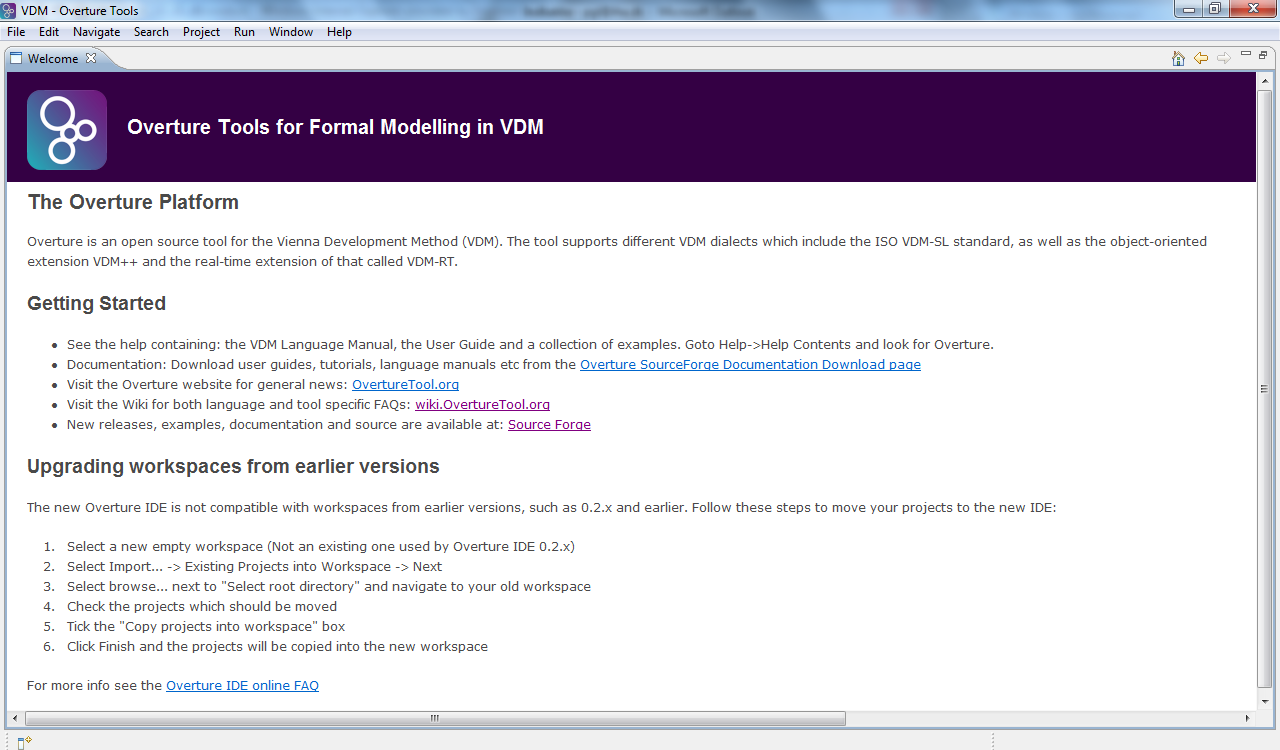
\includegraphics[width=\textwidth]{screenDumps/welcomeWindow}
  \caption{The Overture Welcome Screen}
  \label{fig:userguire:welcomeWindow}
\end{center}
\end{figure}

Large libraries of sample VDM-SL, VDM++ and VDM-RT models are available
and can be downloaded from SourceForge under the
\texttt{files/Examples} section using the URL\footnote{The library
  files are intended to be used with Eclipse, but can also be opened with
  file compression programs like \texttt{Winrar} on Windows}:
\begin{quote}
\url{https://sourceforge.net/projects/overture/files/Examples/}
\end{quote}
Such existing projects can be imported into Overture as described in
section~\ref{subsec:importproj}. 

\chapter{Using the VDM Perspective}\label{sec:vdmsupport}

\section{Understanding Eclipse Terminology}

Eclipse is an open source platform based around a
\emph{workbench}\index{workbench} that provides a common look and feel
to a large collection of extension products. If you are
familiar with one Eclipse product, you will generally find it easy to start
using other products that use the same workbench. The Eclipse workbench
consists of several panels known as \emph{views}\index{view}, such as
those shown in Figure~\ref{fig:userguire:OverturePerspective}.
A particular arrangement of views
is called a \emph{perspective}\index{perspective}\index{perspective!VDM}, for example
Figure~\ref{fig:userguire:OverturePerspective} shows the standard
VDM perspective. This consists of a set of views for managing
Overture projects and viewing and editing files in a
project. Different perspectives are available in Overture as will be
described later, but for the moment think of a perspective as a
useful composition of views for conducting a particular task.

\begin{figure}[!h]
\begin{center}
  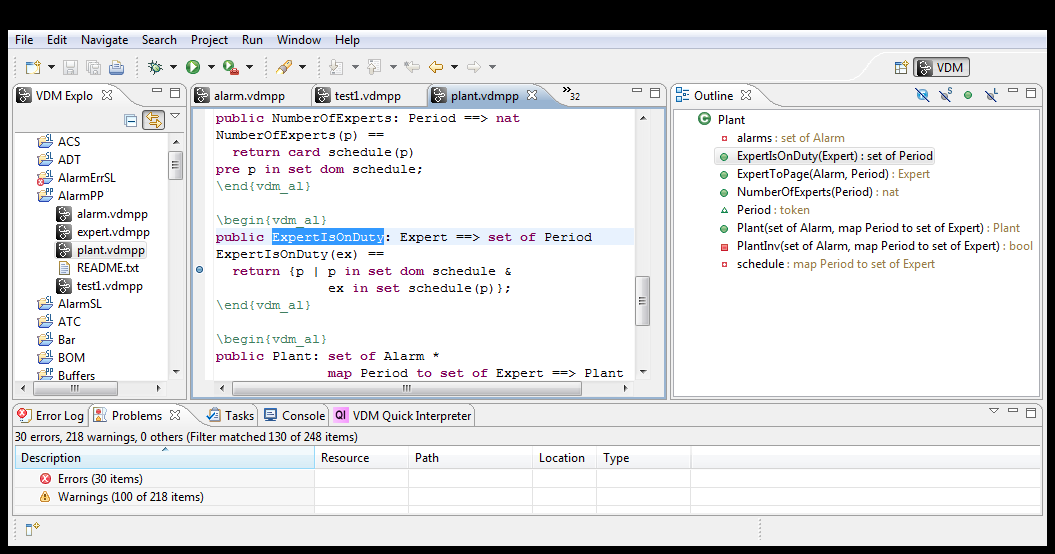
\includegraphics[width=\textwidth]{figures/OverturePerspective}
  \caption[labelInTOC]{The VDM Perspective}
  \label{fig:userguire:OverturePerspective}
\end{center}
\end{figure}

The \emph{VDM Explorer}\index{explorer} view lets you create, select, 
and delete Overture projects and navigate between the files in these 
projects, as well as adding new files to existing projects. A new VDM
project is created choosing the \emph{File} $ \rightarrow$ \emph{New}
$\rightarrow$ \emph{Project} option which results in the dialog shown in
Figure~\ref{fig:userguide:newOvertureProjectSL}. Select
the desired VDM dialect and press \emph{Next}. Finally, the project
needs to be given a name. Click \texttt{Finish} to create the project.
Depending upon the dialect of VDM used in a given project,
a corresponding Overture \emph{Editor} view will be available to edit the files of
your new project. Dialect editors are sensitive to the keywords used in
each particular dialect, and simplify the task of working on the
specification.

\begin{figure}[!h]
\begin{center}
  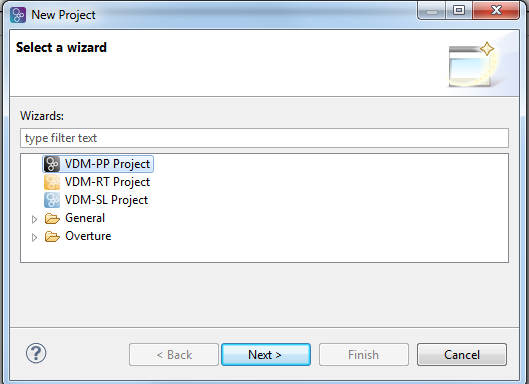
\includegraphics[width=2.5in]{figures/newovertureSLproject}
  \caption[labelInTOC]{Creating a New VDM Project}
  \label{fig:userguide:newOvertureProjectSL}
\end{center}
\end{figure}


The \emph{Outline}\index{outline} view, on the right hand side of 
Figure~\ref{fig:userguire:OverturePerspective}, presents an outline of
the file selected
in the editor. The outline shows all VDM definitions, such as
state definitions, values, types, functions and operations. The
type of each definition is also shown in the view and the colour of
the icons in front of the names indicates the accessibility of each
definition. Red is
used for private definitions, yellow for protected definitions and
green for public definitions. Triangles are used for
type definitions, small squares are used for values, state components
and instance variables, functions and operations are represented by
larger circles and squares, permission predicates are shown with small
lock symbols and traces are shown with a
``\texttt{T}''. Functions have a small ``\texttt{F}'' superscript over the
icons and static definitions have a small ``\texttt{S}'' superscript.
Record types have a small arrow in front of the
icon, and if that is clicked the fields of the record can be seen.
Figure~\ref{fig:OutlineIcons} illustrates the different outline icons.
At the top of the view there are buttons to filter what is displayed,
for instance it is possible to hide non-public members.

\begin{figure}[!htb]
\begin{center}
  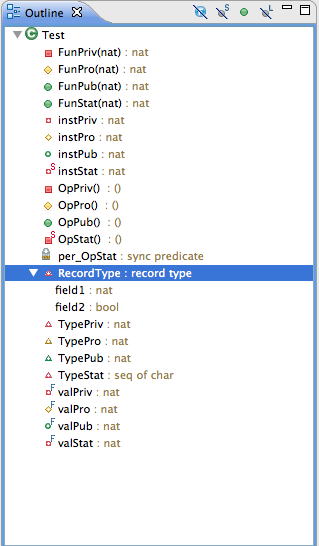
\includegraphics[width=2.5in]{figures/OutlineIcons}
  \caption[labelInTOC]{Icons in the Outline View}
  \label{fig:OutlineIcons}
\end{center}
\end{figure}

Clicking on the name of a definition in the outline will navigate to
the definition and highlight the name in the Editor view.

The \emph{Problems}\index{problems} view at the bottom of 
Figure~\ref{fig:userguire:OverturePerspective} displays 
information messages about the projects you are
working on, such as warnings and syntax or type checking errors.

The \emph{VDM Quick Interpreter}\index{quick interpreter}
view has a small command-line at the bottom where a plain VDM expression
(not depending upon the definitions in the VDM model you are working
with but for that you can use the ``Console'' launch mode explained in
Section~\ref{sec:launchmodes}) can be
entered. When return is pressed, the expression will be evaluated and
the result shown above the command-line.

Most of the other features of the workbench, such as the menus and
toolbars, are similar to other Eclipse applications, with the exception 
of a special menu with Overture specific functionality.

\section{Additional Eclipse Features Applicable in Overture}

\subsection{Opening and Closing Projects}

To de-clutter the workspace and reduce the risk of accidental changes,
it may be helpful to close projects that are not used being worked on.
This can be done by right clicking such projects and then selecting the
\emph{Close Project} entry in the menu. Projects can similarly be re-opened
using the same menu.\index{project!open}\index{project!close} 
 
%\begin{figure}[!htb]
%\begin{center}
%  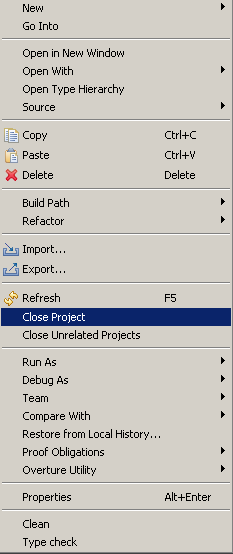
\includegraphics[width=2in]{screenDumps/closeproject}
%  \caption[labelInTOC]{Closing a Project}
%  \label{fig:closeproject}
%\end{center}
%\end{figure}

\subsection{Adding Additional VDM File Extensions}

It is possible to associate additional or different filename extensions with a
particular VDM dialect editor, instead of the standard {\ttfamily .vdmsl},
{\ttfamily .vdmpp} and {\ttfamily .vdmrt}. This is done using the \emph{Window}
$\rightarrow$ \emph{Preferences} menu. Click the Add
button for the appropriate content type.\index{file extension}

\begin{figure}[!htb]
\begin{center}
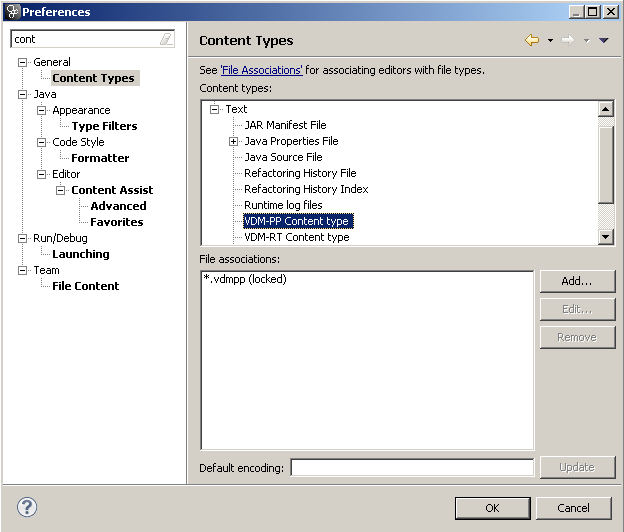
\includegraphics[width=0.6\textwidth]{screenDumps/contentstypes}
\caption{Adding Additional Contents Types\label{fig:ContentsTypes}}
\end{center}
\end{figure}

\subsection{Filtering Project Contents}

It is possible to filter out certain file types from the VDM Explorer view.
This is done by clicking the small downward pointing arrow at the top
right-most corner of the view. See
Figure~\ref{fig:filteringfiles}. The \emph{Filters...} option allows
various files or directories to be hidden, including
directories that have no source files.

\begin{figure}[!htb]
\begin{center}
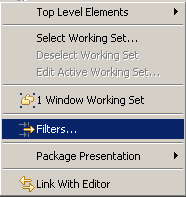
\includegraphics[width=0.4\textwidth]{screenDumps/filteringfiles}
\caption{Filtering Directories without source files\label{fig:filteringfiles}}
\end{center}
\end{figure}

\subsection{Including line numbers in the Editor}

If line numbers\index{line number} are required in the dialect
editors, right click in the left-hand margin
of the editor and select \texttt{show line numbers} as shown in
Figure~\ref{fig:linenumbers}.\index{line numbers} Note that the current
line number and cursor position are displayed in the eclipse status
bar, at the bottom of the workspace, when an editor has focus.

\begin{figure}[!htb]
\begin{center}
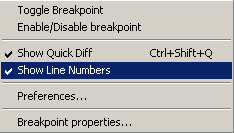
\includegraphics[width=0.4\textwidth]{screenDumps/linenumbers}
\caption{Adding Line Numbers in Editor\label{fig:linenumbers}}
\end{center}
\end{figure}

%\subsection{Adding external plug-ins to Overture IDE}

%The Overture IDE is build as a RCP\footnote{Rich Client Platform} and
%there no update manager is included -- external plug-ins can
%still be manually installed though. To install a plug-in there are two
%things which needs to be done:
%\begin{enumerate}
%\item Copy the plug-in jar or jars into the plugin folder of the Overture IDE installation; and
%\item Add the plug-in jar file names to the \texttt{osgi.bundles} in the config.ini file which is found under the folder configuration.
%\end{enumerate}

%After the steps above have been performed, the IDE can be started and the new plug-ins will be available. (Remember to include all depended plug-ins which is not already a part of the Overture IDE).

%For example, in order to add SVN support to the Overture IDE you simply have to:
%\begin{enumerate}
%\item Fetch the update site jars from \url{http://subclipse.tigris.org/} under \emph{Download and Install} and select \emph{Zipped downloads}. The latest version demonstrated in this guide is site-1.6.10.zip.
%\item Copy the features and plugins folders into the Overture IDE folder, merging them with the ones of Overture. 
%\item Then add the plugins to the \texttt{osgi.bundles} in the \texttt{confi.ini} file separated by comma.
%\begin{itemize}
%\item \url{org.tigris.subversion.clientadapter}
%\item \url{org.tigris.subversion.clientadapter\_1.6.10.jar}
%\item \url{org.tigris.subversion.clientadapter.javahl}
%\item \url{org.tigris.subversion.clientadapter.javahl\_1.6.9.3.jar}
%\item \url{org.tigris.subversion.clientadapter.javahl.win32}
%\item \url{org.tigris.subversion.clientadapter.javahl.win32\_1.6.9}
%\item \url{org.tigris.subversion.subclipse.core}
%\item \url{org.tigris.subversion.subclipse.core\_1.6.10.jar}
%\item \url{org.tigris.subversion.subclipse.doc}
%\item \url{org.tigris.subversion.subclipse.doc\_1.3.0.jar}
%\item \url{org.tigris.subversion.subclipse.graph}
%\item \url{org.tigris.subversion.subclipse.graph\_1.0.7.jar}
%\item \url{org.tigris.subversion.subclipse.ui}
%\item \url{org.tigris.subversion.subclipse.ui\_1.6.10.jar}
%\end{itemize}
%When the steps above are completed the Overture IDE can be started and SVN support will be available.
%\end{enumerate}

\chapter{Managing Overture Projects}\label{sec:projects}

\section{Importing Overture Projects}\label{subsec:importproj}

It is possible to import Overture projects by
right-clicking in the Explorer view and selecting \emph{Import}, followed
by \emph{General} $\rightarrow$ \emph{Existing Projects into
  Workspace}.  In this way the projects from \texttt{.zip} files
mentioned in Chapter~\ref{sec:install} can be imported very
easily.\index{project!import}  

\section{Creating a New Overture Project}

Follow these steps to create a new Overture project:

\begin{enumerate}
	\item Create a new project by choosing \emph{File}
          $\rightarrow$ \emph{New} $\rightarrow$ \emph{Project}
          $\rightarrow$ \emph{Overture}; \index{project!create}
	\item Select the VDM dialect you wish to use (VDM-SL, VDM-PP
          or VDM-RT);\index{VDM dialect}
	\item Click \emph{Next};
         \item Type in a project name;
	\item Choose whether you would like the contents of the new
          project to be in your workspace or outside
          (browse to the appropriate directory); and
    \item Click	the Finish button (see Figure~\ref{fig:CreateProjectWizard}).
\end{enumerate}

\begin{figure}[!htb]
	\begin{center}
	  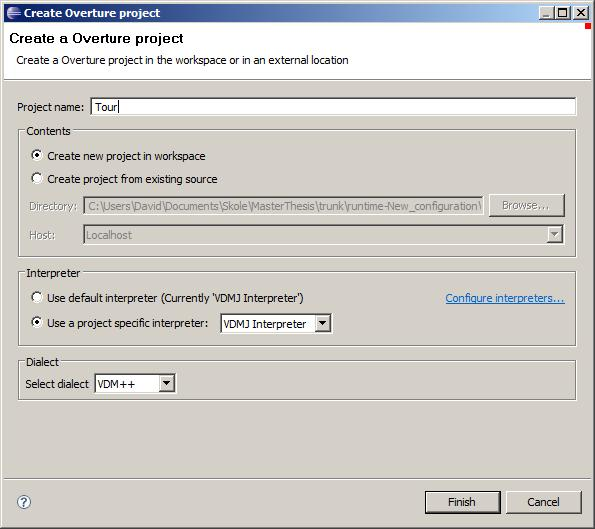
\includegraphics[scale=0.8]{figures/CreateProjectWizard}
	  \caption[Create Project Wizard]{Create Project Wizard}
	  \label{fig:CreateProjectWizard}
	\end{center}
\end{figure}

%%%%%%%%%%%%%%%%%%%%%%%%%%%%%%%%%%
%  Creating a new file
%%%%%%%%%%%%%%%%%%%%%%%%%%%%%%%%%%

\section{Creating Files}

Switching to the VDM perspective will change the layout of the user
interface to focus on VDM development. To change perspective, go to the menu 
\emph{Window} $\rightarrow$ \emph{Open perspective} $\rightarrow$
\emph{Other...} and choose the VDM perspective.
From the this perspective you can create files
using one of the following methods:

\begin{enumerate}
  \item Choose \emph{File} $\rightarrow$ \emph{New} $\rightarrow$
    \emph{VDM-SL Module}\index{creating!VDM-SL module} or 
    \emph{VDM-PP Class}\index{creating!VDM++ class} or 
    \emph{VDM-RT Class}\index{creating!VDM-RT class} or
  \item Right click on the Overture project where you would like to
    add a new file and then choose \emph{New} $\rightarrow$ 
    \emph{VDM-SL Module} or \emph{VDM-PP Class} or \emph{VDM-RT Class}.
\end{enumerate}

In both cases you need to choose a file name and optionally choose a
directory if you do not want to place the file in the home directory of
the chosen Overture project. Then a new file with the appropriate file
extension (according to the chosen dialect, \texttt{.vdmsl},
\texttt{.vdmpp} or \texttt{.vdmrt})\index{vdm file extension} will be
created in the directory. This file will use the appropriate
module/class template to get you started. Naturally, keywords 
that are not required can be deleted from the template.

\section{Adding Standard Libraries}

In addition to adding new empty files it is possible to add existing
standard libraries. This can be done by right-clicking on the project
where the library is to be added and then selecting \emph{New} $\rightarrow$
    \emph{Add VDM Library}. That will make a new window as shown in
    Figure~\ref{fig:NewLibraries}. Here the different standard
    libraries provide different standard functionalities. In the body
    of many of these functions/operations are declared as
    ``{\textbf{\ttfamily is not yet specified}}'' but the actual
    functionality for all of these are hard-coded into Overture so the
    user can get access to this when the respective standard libraries
    are included. This can be
    summarised as:

\begin{description}
\item[IO:] This library provides functionality for input and output
  from/to files and the standard console. 
\item[Math:] This library provides functionality for standard
  mathematical functions such as sine and cosine.
\item[Util:] This library provides functionality for converting
  different kind of VDM values mainly to and from files and strings.
\item[CSV:] This library is an extension of the IO library which
  provides additional functionality for saving and reading VDM values
  to/from comma seperate format used by excel spreadsheets. 
\item[VDM-Unit:] This library provides functionality for unit testing
  of VDM models similar to the well-known JUnit library.
\end{description}

\begin{figure}[!htb]
	\begin{center}
	  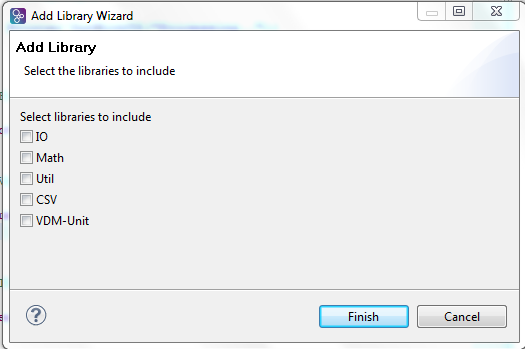
\includegraphics[scale=0.8]{figures/NewLibraries}
	  \caption[Adding New Libraries]{Adding New Libraries}
	  \label{fig:NewLibraries}
	\end{center}
\end{figure}

These libraries are available for all VDM dialects also when a flat
VDM-SL specification is used.

\section{Setting Project Options}\label{subsec:options}

There are various VDM
specific settings for an Overture project. You can change these by
selecting a project
in the \emph{Explorer} view and then right clicking and selecting
\emph{Properties}. See Figure~\ref{fig:VDMSettings}. The options 
that can be set for each VDM project are:\index{project!options}

\begin{figure}[!hbt]
\begin{center}
  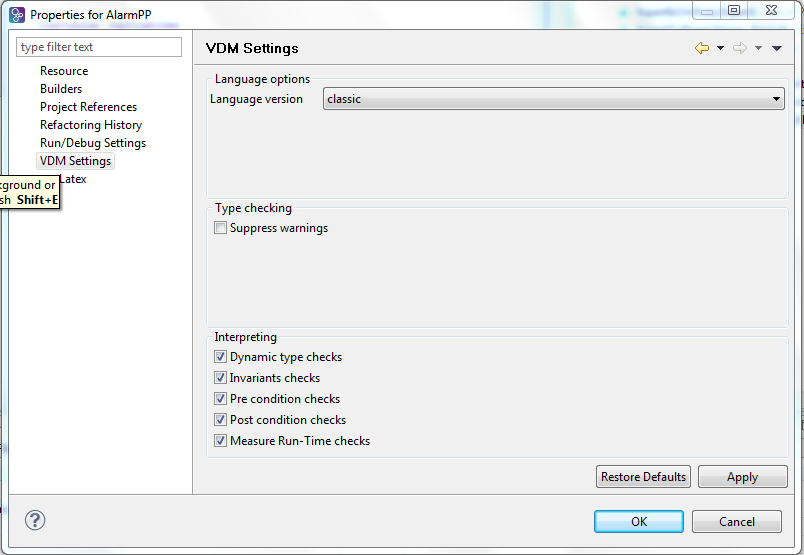
\includegraphics[width=\textwidth]{screendumps/projectsettings}
  \caption[Overture Project Settings]{Overture Project Settings}
  \label{fig:VDMSettings}
\end{center}
\end{figure}

\begin{description}
\item[Language version:] Here the default is to use the
  \emph{classic} version which is similar to that used in
  VDMTools. Alternatively you can select VDM-10 which
  is a new improved (but not necessarily backwards compatible) version of
  the VDM dialects developed by the Overture Language Board. 
\item[Suppress type checking warnings:] Warnings are enabled
  by default but you can change it here.
\end{description}

Overture allows VDM specifications to be embedded in \LaTeX\ files that
form part of the documentation of a project as seen in
Figure~\ref{fig:VDMSettingsLatex}. The project settings allow you
to define a main \LaTeX\ file for the project, and define the order in which the
different VDM source files shall be included. Note that if the
``\texttt{Insert coverage tables}'' and ``\texttt{Mark coverage}''
options are selected the \LaTeX\ pretty printing will include test
coverage information as well as provide test coverage tables for each
class/module in the VDM model. It is also possible to define your own
main document instead of making use of the standard one suggested by
Overture (which is the name of the project followed by \texttt{.tex}).

\begin{figure}[!hbt]
\begin{center}
  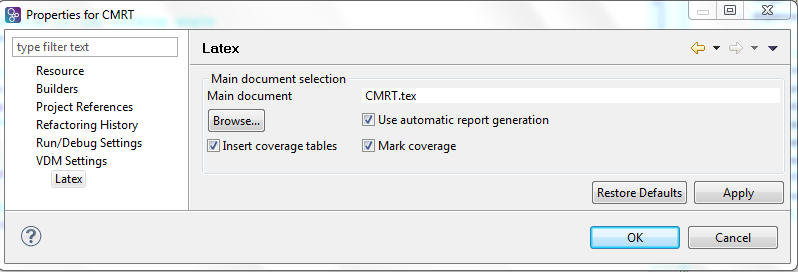
\includegraphics[width=\textwidth]{screendumps/projectsettingslatex}
  \caption[Overture Project Settings]{Overture Project Settings for \LaTeX}
  \label{fig:VDMSettingsLatex}
\end{center}
\end{figure}

It is also possible to set various preferences that apply to
all projects. This is done in the general VDM preferences dialog under
\emph{Window} $\rightarrow$ \emph{Preferences} $\rightarrow$
\emph{VDM}. Here, for example, it is possible to link projects to
VDMTools if you have the appropriate CSK executables installed on
the computer. Figure~\ref{fig:CSKPreferences} shows how it is possible to
set up paths to the corresponding VDMTools executables. If these paths have
been set, it is possible to right click on a project in the VDM
Explorer view and select \emph{VDM Tools} $\rightarrow$
\emph{Open project in VDMTools}. Then a project file for VDMTools
will automatically be generated with all the files from the Overture project
and VDMTools will be opened. The \emph{Preferences} dialog also
allows you to switch off continuous syntax checking while editing and
to set the path to \emph{pdflatex} if this is not automatically
visible from the Overture application. Finally it is possible to 
manage VDM templates, but that is described in Section~\ref{sec:templates}. 

\begin{figure}[!hbt]
\begin{center}
  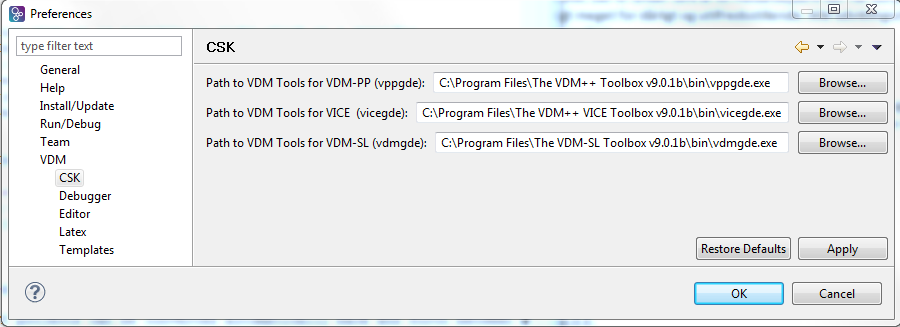
\includegraphics[width=\textwidth]{screendumps/CSKPreferences}
  \caption{Overture Preferences for connctions to VDMTools}
  \label{fig:CSKPreferences}
\end{center}
\end{figure}

\chapter{Editing VDM Models}\label{sec:editVDM}

\section{VDM Dialect Editors}

VDM model files are always changed in the dialect Editor view. Syntax checking
is carried out continuously as source files are
changed (even before the files are saved). Whenever files are saved, assuming
there are no syntax errors, a full type check of the \emph{entire} VDM model is
performed.
Problems and warnings will be listed in the Problems view as well as
being highlighted directly in the Editor view where the problems have been
identified.


\section{Using Templates}\label{sec:templates}

Eclipse templates can be particularly useful when writing VDM models. If you
press \textit{CTRL+space} after typing the first few characters of a template name,
Overture will offer a proposal. For example, if you type ''fun'' followed
by \textit{CTRL+space}, the IDE will propose the use of an implicit or explicit
function template as shown in Figure~\ref{fig:functionTemplate}. The IDE includes
several templates: cases, quantifications, functions (explicit/implicit),
operations (explicit/implicit) and many more. The use of templates makes it much
easier for users to create models, even if they are not deeply familiar
with the VDM syntax.

\begin{figure}
\begin{center}
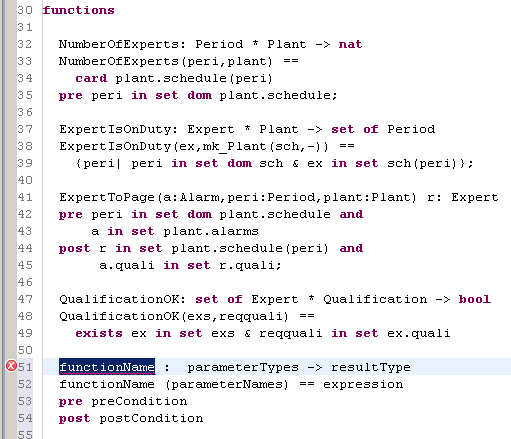
\includegraphics[width=4in]{figures/FunctionTemplate}
\caption{Explicit function template}
\label{fig:functionTemplate}
\end{center}
\end{figure}

It is possible to adjust or add to the templates defined in 
Overture. This can be done in the general VDM preferences under
\emph{Window} $\rightarrow$ \emph{Preferences} $\rightarrow$ \emph{VDM}
$\rightarrow$ \emph{Templates}. Figure~\ref{fig:Templatepreferences} shows
how the template for ``cases'' expressions is defined in Overture. Note
that new templates can be added and the existing ones can be
edited or removed. A full list of the
standard Overture templates is available in Appendix~\ref{app:templates}.

\begin{figure}
\begin{center}
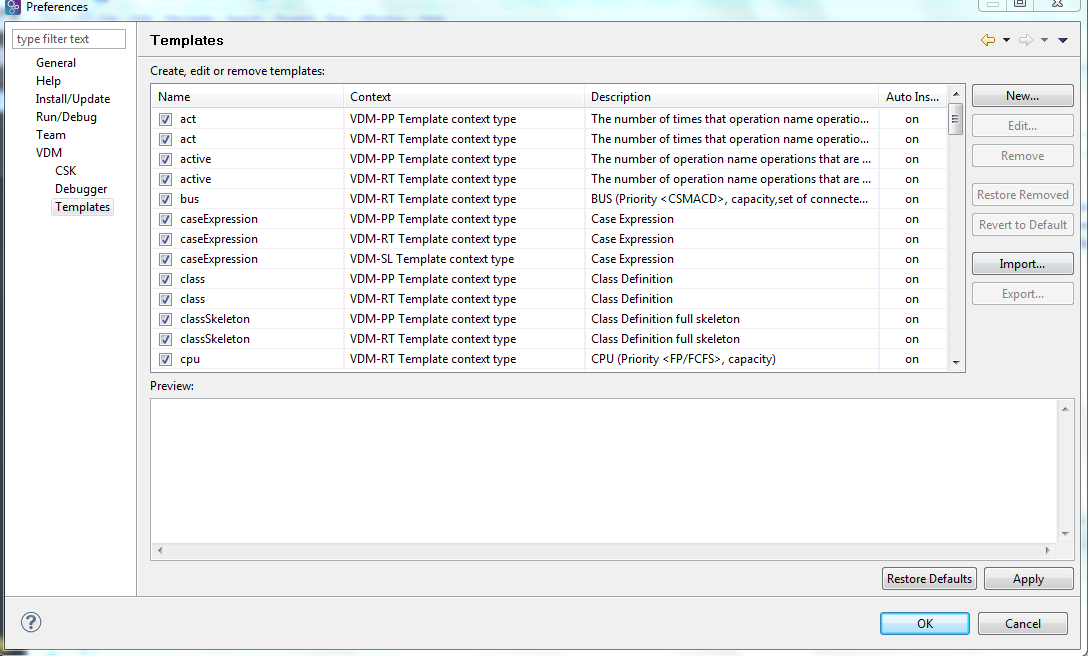
\includegraphics[width=4in]{screendumps/templatesRT}
\caption{Adjusting templates for Overture}
\label{fig:Templatepreferences}
\end{center}
\end{figure}

\chapter{Interpretation and Debugging in Overture}\label{sec:debug}

This section describes how to run and debug a model using the Overture IDE. 

\section{Run and Debug Launch Configurations}\label{sec:launchmodes}

To execute or debug a VDM model, you must first create a launch
configuration\index{debug configuration}. To do this, go to the main Run menu
and select \emph{Run} $\rightarrow $ \emph{Run Configurations}. Select the type of
project you want to launch, click the New icon to
create a new launch specification of that type and give it a name. The
launch dialog requires you to identify the VDM project name,
the class/module name and the initial operation/function to call in that
class/module. Figure~\ref{fig:userguide:launchconfig} shows a launch
dialog. The standard Eclipse strategy is the launch mode called
``Entry point'' and then you simply click 
the Browse button and it will let you select a project from
those available in the workspace. Clicking the Search button will search the chosen
project for classes and modules to select a public operation or function from.
If the chosen operation or function has parameters, the types and names of those
parameters will be copied into the Operation box - these \emph{must} be replaced with
valid argument values\footnote{You will see type checking errors at the top of the
dialog if you do not do this, such as "Error 3063: Too few arguments in ..."}.

However, there are other launch mode possibilities here as
well.\index{launch configuration mode} The
``Remote Control'' launch mode is advanced but it is explained in mode
detail in Section~\ref{sec:javalibs}. The ``Console'' launch mode
enables you to get a special debug console where you can enter
multiple entry points (one after another) instead of deciding upon the
single entry point at launch time\footnote{Those familiar with
  VDMTools will recognise this functionaility as initialising a
  specific VDM model and then having a prompt where different
  expressions can be evaluated making use of the definitions from the model.}.
The commands that can be used in the ``Console'' view correspond to
the commands you can give in VDMJ when it has been started in
interpreter mode (see Section~\ref{sec:commandlineinterpreter}).

Your new launch configuration can be started immediately by clicking the \emph{Run}
button at the bottom of the dialog. Alternatively, the configuration can simply be
saved by clicking \emph{Apply}. Once a launch configuration has been defined, it
can be re-run at any time by using the small downward arrow next to the run or
debug icons (
\includegraphics[width=0.03\textwidth]{icons/debuggericon})
in the IDE toolbar.

A launch configuration can either be started normally, which will simply evaluate
the expression given and stop, or it can be started in debug mode, which will
stop the evaluation at any breakpoints you may have set. The same launch configuration
can be used for either purpose, though by default those created through the
\emph{Run Configurations} dialog will appear in the favourites list under the
\emph{Run} toolbar icon. Similarly, a launch configuration created under the
\emph{Debug Configurations} dialog will appear under the favourites of the
debug toolbar icon. You can control which icons display the launch configuration
in the \emph{Common} tab on the dialog. This is standard Eclipse behaviour.


\begin{figure}[htp]
\begin{center}
  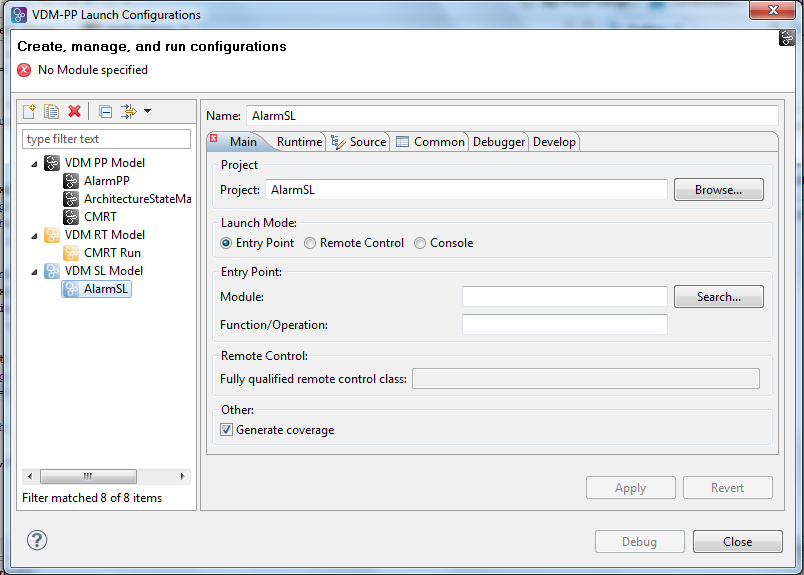
\includegraphics[width=380px]{screenDumps/launchconfig}
  \caption{The launch configuration dialog}
  \label{fig:userguide:launchconfig}
\end{center}
\end{figure}

Whenever a launch configuration is started up it is also possible to
decide upon which additional run-time checks to carry out. Per default
all possible run-time checks are swiched on but if desired (some of)
these can be swiched off using the ``Runtime'' pane (see
Figure~\ref{fig:userguide:launchconfigRToptions}). Note that for
VDM-RT debugging it is also possible to switch off the logging of all
events appearing during the debugging. The different run-time checks
that can be performed are:

\begin{description}
\item[Dynamic type checks:] This is an option for the interpreter (default on) 
  to continuously type check  values during interpretation of a VDM model.
  It is possible to switch off the check here.
\item[Invariant checks:] This is an option for the interpreter (default on) 
  to continuously check both state and type invariants.
  It is possible to switch off
  this check here, but note that option requires dynamic type
  checking also to be switched off.
\item[Pre condition checks:] This is an option for the interpreter (default on) 
  to continuously check pre-conditions for all functions and operations
  during interpretation of a VDM model. It is possible to switch off
  this check here.
\item[Post condition checks:] This is an option for the interpreter (default on) 
  to continuously check post-conditions for all functions and operations
  during interpretation of a VDM model. It is possible to switch off
  this check here.
\item[Measure checks:] This is an option for the interpreter (default
  on) to continuously check recursive functions, for which a
  measure function has been defined. It is possible to switch off this
  check here.
\end{description}

In the launch
configuration the ``Debug'' pane shown in
Figure~\ref{fig:userguide:launchconfigSpecialOptions} can also be
useful in rare cases where one have particular deep recursion for
example. this is an advanced setting where one can decide the
arguments given to the Java virtual machine for allocation of maximum
amounts of space per thread in a VDM model. However, this option is
rarely used.

\begin{figure}[htp]
\begin{center}
  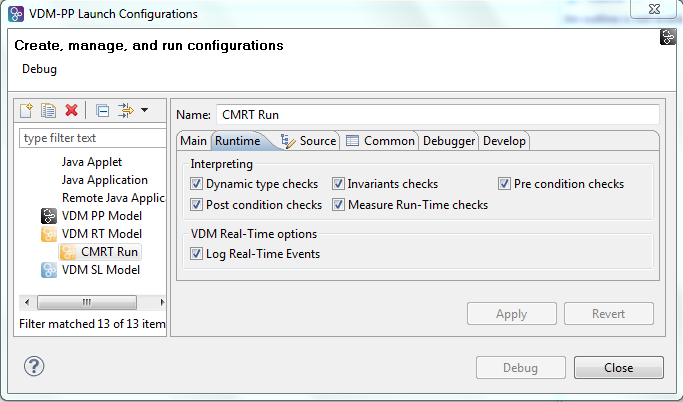
\includegraphics[width=380px]{screenDumps/launchconfigRToptions}
  \caption{The launch configuration dialog}
  \label{fig:userguide:launchconfigRToptions}
\end{center}
\end{figure}

\begin{figure}[htp]
\begin{center}
  \includegraphics[width=380px]{screenDumps/launchconfigSpecialOptions}
  \caption{The launch configuration dialog}
  \label{fig:userguide:launchconfigSpecialOptions}
\end{center}
\end{figure}

\section{The Debug Perspective}

The Debug Perspective\index{debug perspective} contains all the views
commonly needed for debugging in VDM. Breakpoints can easily be set in the
model by double clicking in the left margin of the Editor view at the chosen
line. When the debugger reaches the location of a breakpoint and stops, you can
inspect the values of different identifiers and step through the VDM model 
line by line.\index{perspective!debug}
 
The Debug Perspective is illustrated in Figure~\ref{fig:userguide:DebuggingVDM}

\begin{figure}[htp]
\begin{center}
  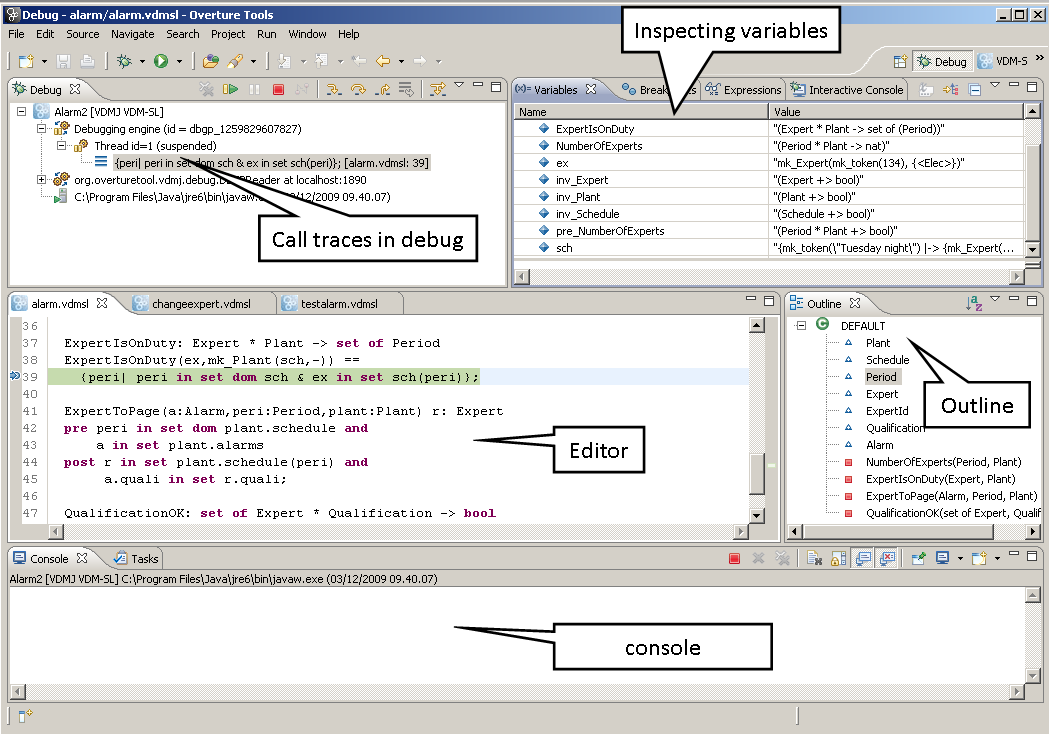
\includegraphics[width=380px]{figures/DebuggingVDM}
  \caption[Debugging perspective]{Debugging perspective}
  \label{fig:userguide:DebuggingVDM}
\end{center}
\end{figure}

%The \emph{Debug view} is located in the upper left corner in the Debug
%perspective. The Debug view shows all running models and the call stacks
%belonging to them. It also shows whether a given model is stopped, suspended or
%running. All threads are also shown, along with their running status. It is
%possible to switch between threads from the Debug view.

\begin{table}
\begin{center}
\caption{Overture debugging buttons\label{tab:debugButtons}}
\begin{tabular}{|l|l|}\hline \hline
\textbf{Button} & \textbf{Explanation} \\ \hline

\includegraphics[width=0.03\textwidth]{figures/resume} & Resume
debugging\index{icon!resume debugging} \\

\includegraphics[width=0.03\textwidth]{figures/suspend} & Suspend
debugging\index{icon!suspend debugging}\\

\includegraphics[width=0.03\textwidth]{figures/terminate} & Terminate
debugging\index{icon!terminate debugging}\\

\includegraphics[width=0.03\textwidth]{figures/stepinto} & Step
into\index{icon!step into}\\

\includegraphics[width=0.03\textwidth]{figures/stepover} & Step
over\index{icon!step over} \\

\includegraphics[width=0.03\textwidth]{figures/stepreturn} & Step
return\index{icon!step return}\\

\includegraphics[width=0.03\textwidth]{figures/stepbystep} & Use step
filters\index{icon!use step filters}\\
\hline \hline
\end{tabular}
\end{center}
\end{table}

\subsection{The Debug View}

The \emph{Debug} view is located in the upper left corner in the Debug perspective --
see Figure~\ref{fig:userguide:DebuggingVDM}. The view shows all running
models and whether a given model is stopped, suspended or running.
It shows the call stack of models that are suspended, and for VDM++ and VDM-RT stacks
for all threads are shown.
At the top of the view, there are buttons
for debugging such as: stop, step into, step over, resume, etc. (see
Table~\ref{tab:debugButtons}). Note that in case a multi-threaded VDM
model is debugged it is possible in this view to change to another
thread to inspect where it is currently and inspect the local
variables at that thread since they are all stopped when a breakpoint
is reached.

\subsection{The Variables View}
 
The \emph{Variables} view shows all the variables in a thread context, allowing them to be
examined after a breakpoint (or an error) has been reached. The variables and their values are
automatically updated when stepping through a model. The view is
located in the upper right hand corner in the Debug perspective. It is
possible to inspect compound variables, expand nested structures and
so on. Note that when you stop at a permission predicate it is also
possible to see the value of the relevant history counters (in
Figure~\ref{fig:userguide:DebuggingVDM} \texttt{\#fin(ClientSend)} and
\texttt{\#fin(ServerListen)}). By right-clicking on a variable it is
possible to select a ``watch point''. As a result a window like
Figure~\ref{fig:watchpoint} will occur. Using this it is possible to
watch the value of such a variable easily whenever a new stop is
reached in the debugging process.

\begin{figure}[htp]
\begin{center}
  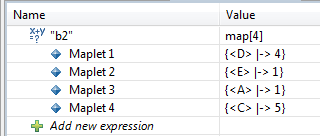
\includegraphics[width=.5\textwidth]{screenDumps/watchpoint}
  \caption{Example of a watchpoint}
  \label{fig:watchpoint}
\end{center}
\end{figure}

\subsection{The Breakpoints View}

Breakpoints can be added in any perspective from the Editor view\footnote{Note that
breakpoints can only be set on lines that contain executable code.}.
The debug perspective also has a \emph{Breakpoints} view that lists all current
breakpoints, allowing you to navigate easily to the location of a given breakpoint,
disable it or delete it. The view is located in
the same panel as the Variables view in the upper right hand corner.


\subsection{Conditional Breakpoints}
\label{sec:userguide:breakpoints}

Breakpoints can be conditional. This is a powerful feature for the
developer since it allows you to specify a conditional expression 
which has to be true for the debugger to stop at the given breakpoint.
As well as using an expression, a conditional breakpoint may specify a
hit count and whether the breakpoint should stop when the hit count is
equal to, greater than, or a multiple of the given value, or a general
expression using the variables in scope at the breakpoint.

A normal breakpoint can be made conditional by right clicking on the breakpoint
mark in the Editor view\footnote{Note this is not possible from the Breakpoint view}
and selecting \emph{Breakpoint Properties}. This opens a dialog like the one shown in
Figure~\ref{fig:userguide:BreakpointConditional}.

\begin{figure}[htp]
\begin{center}
  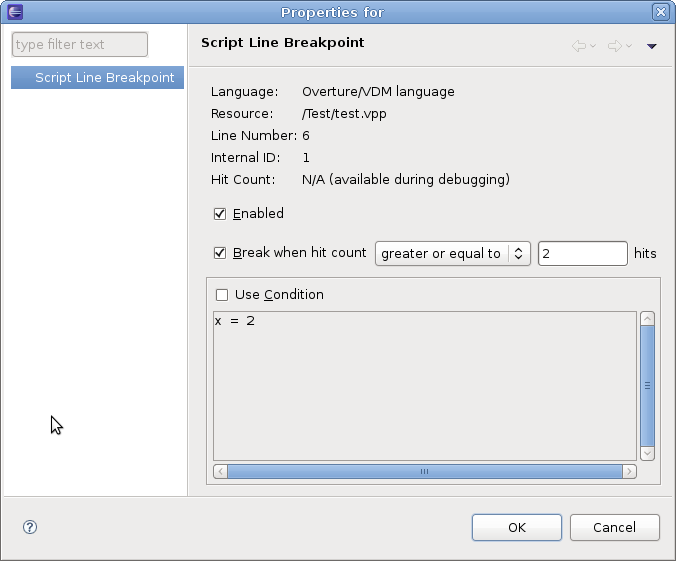
\includegraphics[width=.6\textwidth]{figures/Breakpointconditional}
  \caption{Conditional breakpoint options}
  \label{fig:userguide:BreakpointConditional}
\end{center}
\end{figure}

\subsection{The Expressions View}

The \emph{Expressions} view allows you to define expressions that are evaluated
whenever the debugger stops.
Watched expressions can be added to the view directly, or created by selecting \emph{Watch}
when right-clicking a variable in the Variables view. It is also possible to edit existing
expressions. The view sits in the same panel as the Breakpoints view and
the Variables view.

\chapter{Collecting Test Coverage Information}\label{sec:testcoverage}

When a VDM model is being interpreted, it is possible to automatically collect
test coverage information. Test coverage measurements help you to see how well a
given test suite\index{Test Coverage!Test suite} exercises your VDM model.

In order to enable the collection of test coverage data, go to the debug launch 
configuration and select the \emph{Generate coverage} option. After
running this configuration, a new file with a \texttt{.cov} extension will be created for 
each file in the project. These files are written into a project subfolder named
\texttt{generated/coverage/<date and time>}. Double-clicking the \texttt{.cov} files
will open a special editor window that displays the source with coverage
coloured in red/green (red is executable but not covered). Alternatively, a PDF file
containing the entire model with coloured test coverage summarised for all runs
can be generated 
by right-clicking on the project name and selecting \emph{Latex} $\rightarrow$ 
\emph{Latex Coverage}.

\chapter{Pretty Printing to \LaTeX}\label{sec:prettyprint}

%Include \texttt{overture.tex} which among other things makes use of the
%\texttt{times.cls} and \texttt{listings.cls} style classes. This enables
%the use of the standard \texttt{lstlisting} environment for type setting
%source text and display it in a fixed width font where all VDM keywords
%are typeset in bold.

It is possible to use literate programming/specification \cite{Johnson96} with
Overture just as you can with VDMTools. To take advantage of this,
you need to use the \LaTeX\ text processing system with
plain VDM models mixed with textual documentation.  The VDM model parts must be
enclosed within ``\verb+\begin{vdm_al}+'' and ``\verb+\end{vdm_al}+''. The
text-parts outside these specification blocks are ignored by the VDM parser,
though note that each source file must start with a recognizable \LaTeX\
construct: a \verb+\documentclass, \section, \subsection+ or a \LaTeX\ comment.


\chapter{Managing Proof Obligations}\label{sec:POmanagement}

In all VDM dialects, Overture can identify places where run-time errors
\emph{could} potentially occur if the model was to be executed. The analysis of
these areas can be considered
as a complement to the static type checking that is performed automatically.
Type checking accepts specifications that are \emph{possibly} correct, but
we also want to know the places where the specification could possibly fail.

Unfortunately, it is not always possible to statically check if such
potential problems will \emph{actually} occur at run-time error or not. So Overture
creates \emph{Proof Obligations}\index{proof obligation} for all the places
where run-time errors \emph{could} occur. Each proof obligation (PO)
is formulated as a predicate that must hold at a particular place in the VDM
model if it is error-free, and so it may have particular context information
associated with it. POs can be considered as
constraints that will guarantee the internal integrity of a VDM model if they
are all met. In the long term, it will be possible to prove these constraints
with a proof component in Overture, but this is not yet available.

POs can be divided into different categories\index{proof obligation!categories}
depending upon their nature. The full list of categories can be found in
Appendix~\ref{app:POcategories} along with a short description for
each of them.

The proof obligation generator is invoked either on a VDM project (and
then POs for all the VDM model files will be generated) or for one
selected VDM file. Right-click the project or file in the Explorer view and
then select \emph{Proof Obligations} $\rightarrow$ \emph{Generate Proof
  Obligations}. Overture will change into a special
\emph{Proof Obligations} perspective\index{proof
  obligation!perspective} as shown in
Figure~\ref{fig:POview}.\index{perspective!proof obligation}  

\begin{figure}[htbp]
\begin{center}
\includegraphics[width=\textwidth]{figures/POview}
\caption{The Proof Obligation perspective\label{fig:POview}}
\end{center}
\end{figure}

Note that in the \emph{Proof Obligation Explorer} view, each proof
obligation has four components:
\begin{itemize}
\item A unique number in the list shown;
\item The name of the definition in which the proof obligation is
  located;
\item The proof obligation category (type); and
\item A status field indicating whether the proof obligation is
  trivially correct or would have to be proved by a proof engine.
\end{itemize}

At the top of the \emph{Proof Obligation Explorer} the \emph{Filter proved} button
allows you to filter away all the proof obligations that are trivially
correct.\index{filter proved} 

\chapter{Combinatorial Testing}\label{sec:testing}

In order to better automate the testing process, a notion of
test \emph{traces} has been introduced into VDM++\footnote{Note that this is 
only available for VDM-SL models if the VDM-10 language version has been selected}. 
Traces are effectively regular expressions that can be expanded to a collection of test
cases. Each test case comprises a sequence of operation
calls. If a user defines a trace it is possible to make use of a
special \emph{Combinatorial Testing} perspective to automatically
expand the trace and execute all of the resulting test
cases. Subsequently, the results from the tests can be inspected
and erroneous test cases easily found. You can then fix 
problems and re-run the trace to check they are fixed.

\section{Using the Combinatorial Testing GUI}

The syntax for trace definitions is defined in the VDM-10 Language
Manual.\index{traces}
If you have created a \texttt{traces} entry for a module or class it
can be executed via the \emph{Combinatorial Testing}
perspective\index{combinatorial testing}. See
Figure~\ref{fig:tracesalarm}.\index{perspective!combinatorial testing}

Different icons are used to indicate the verdict in a test
case. These are:
\begin{description}
\item[\hspace{-1.8mm}
\raisebox{-0.8mm}{
\includegraphics[width=0.03\textwidth]{icons/unknownWhiteBG.png}}:]
  This icon is used to indicate that the test case has not yet been
  executed.
\index{icon!not yet executed}
\item[\hspace{-1.8mm}
\raisebox{-0.8mm}{
\includegraphics[width=0.03\textwidth]{icons/okBigWhiteBG.png}}:]
  This icon is used to indicate that the test case has a pass
  verdict.\index{icon!pass verdict}
\item[\hspace{-1.8mm}
\raisebox{-0.8mm}{
\includegraphics[width=0.03\textwidth]{icons/undeterminedBigWhiteBG.png}}:]
  This icon is used to indicate that the test case has an inconclusive
  verdict.\index{icon!inconclusive verdict}
\item[\hspace{-1.8mm}
\raisebox{-0.8mm}{
\includegraphics[width=0.03\textwidth]{icons/faildBigWhiteBG.png}}:]
  This icon is used to indicate that the test case has a fail
  verdict.\index{icon!fail verdict}
\item[\hspace{-1.8mm}
\raisebox{-0.8mm}{
\includegraphics[height=10pt]{screenDumps/skippedIndication.png}}:] 
If any test cases result in a run-time error, other test cases with the
same sequence of calls will be filtered and automatically skipped in the test
execution. The number of skipped test cases is indicated after the number
of test cases for the trace definition name.\index{icon!skipped test case}
\end{description}

\begin{figure}[htbp]
\begin{center}
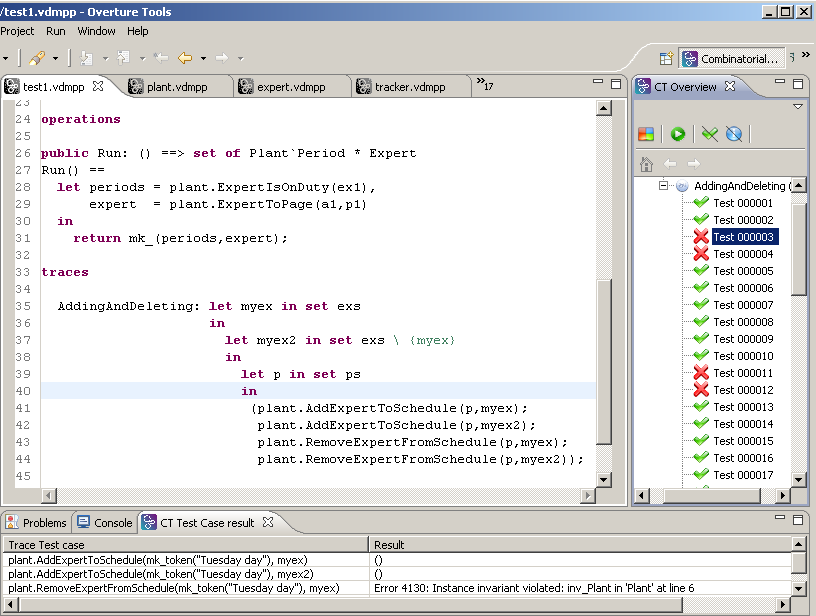
\includegraphics[width=4.5in]{screenDumps/tracesalarm}
\caption{Using Combinatorial Testing\label{fig:tracesalarm}}
\end{center}
\end{figure}

In the CT Overview view, you can right-click on any individual
test case and then execute it with the interpreter (see
Figure~\ref{fig:SendToInterpreter}). This is particularly useful for
failed test cases since the interpreter allows you to step through the
evaluation to the place where it is failing. You can inspect the exact
circumstances of the failure, including the values of the different
variables in scope. 

\begin{figure}[htbp]
\begin{center}
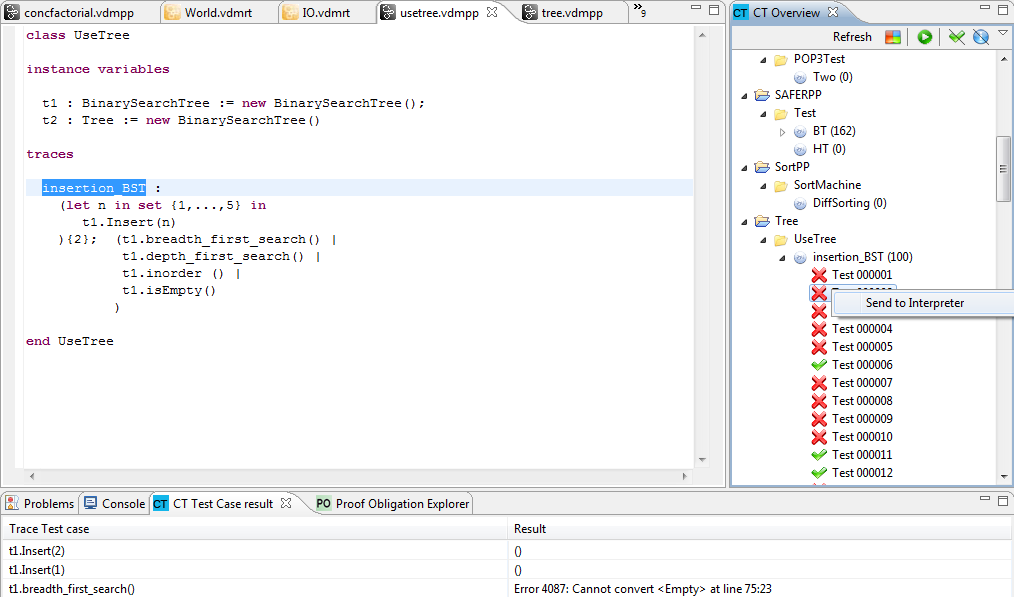
\includegraphics[width=4.5in]{screenDumps/SendToInterpreter}
\caption{Moving test case from Combinatorial Testing to Interpreter\label{fig:SendToInterpreter}}
\end{center}
\end{figure}

\chapter{Mapping VDM++ To and From UML}\label{sec:vdmuml}

VDM++ and VDM-RT projects can be converted automatically back and forth between VDM
and the corresponding UML model\footnote{In the current version of
Overture this feature is somewhat unstable.}. 
Essentially, VDM and UML can be considered
as different views of the same model. A UML model is typically used
to give a graphical overview of the model using class diagrams, and
sequence diagrams can be used to indicate the test scenarios
that a user would like to perform. The VDM model is typically used
to define the implementation and constraints for each class and
is therefore used for detailed semantic analysis.

The exchange between VDM and
UML is done using the XML format called XMI\index{XMI}. At the moment,
Enterprise Architect\index{Exterprise Architect} is the only UML tool
supported. Export from EA is done by selecting the \emph{Project} menu
and \emph{Import/Export} $\rightarrow$ \emph{Export Package
to XMI}. This is illustrated in Figure~\ref{fig:exportfromUML}.

\begin{figure}[htbp]
\begin{center}
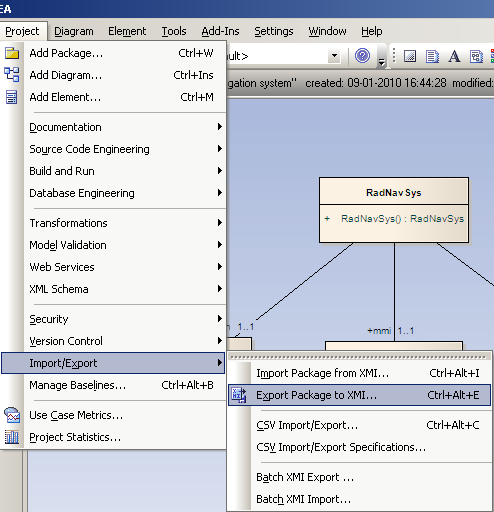
\includegraphics[width=4.5in]{screenDumps/exportfromUML}
\caption{Exporting UML definitions from EA\label{fig:exportfromUML}}
\end{center}
\end{figure}

Importing and exporting a UML model is
an option in the Overture \emph{Explorer} view, where right-clicking
a VDM++ or VDM-RT project gives a submenu for
\emph{UML Transformation}\index{UML transformation}. From here
it is possible to \emph{Import XMI}\index{import XMI} or to
\emph{Export XMI}\index{Export XMI}.

\chapter{Moving from VDM++ to VDM-RT}\label{sec:ToVDMRT}

The methodology for the development of distributed real-time
embedded systems in VDM defines a step where you
move from an initial VDM++ model to a VDM-RT model\cite{Larsen&09b}. This
step is supported by the Overture tool which will convert
a VDM++ project to create the starting point for a new VDM-RT
project. This is done by right-clicking on the VDM++ project to be
converted in the Explorer view, followed by 
the \emph{Clone as VDM-RT} option\index{create real time
  project}. A new VDM-RT project is then automatically
created. It will have the
same name as the original VDM++ project, but with \texttt{VDM\_RT} appended.
Inside the project, all the \texttt{.vdmpp} files will have been converted
to a \texttt{.vdmrt} extension. The original VDM++ project is not
changed at all. So this is simply a quick and easy way to get to the
starting point for a VDM-RT model. You would then manually create
a \texttt{system} class with appropriate declarations of
\texttt{CPU}s and \texttt{BUS}ses and proceed with the real time
model development.
 
\chapter{Analysing and Displaying Logs from VDM-RT Executions}\label{sec:showlog}

Whenever a VDM-RT model is executed, a logfile is created in
a \texttt{generated/logs/<launch>} subfolder with a \texttt{.logrt} extension. The
file name for the logfile indicates the time at which the model was executed,
so it is possible to distinguish multiple runs. Logfiles can be
viewed with the built-in \emph{RealTime Log Viewer},\index{RealTime Log viewer}
by double-clicking the .logrt file in the Explorer view. The log viewer enables
you to explore the simulated system execution in various ways. In
Figure~\ref{fig:userguide:ArchitecturalOverview} the architectural
overview of the system is shown, describing the CPU and BUS topology of
the model.\index{architecture overview}

\begin{figure}[htp]
\begin{center}
  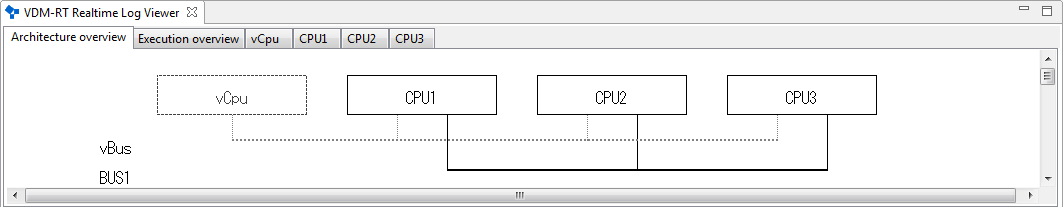
\includegraphics[width=4in]{figures/ArchitectureOverview}
  \caption{Architectural overview}
  \label{fig:userguide:ArchitecturalOverview}
\end{center}
\end{figure}

The log viewer also enables you to get an overview of
the model execution\index{model execution overview} at a system level --
see Figure~\ref{fig:userguide:ExecutionOverview}.
This view shows how the different CPUs\index{CPU} communicate via the
BUSes\index{BUS} of the system. 

\begin{figure}[htp]
\begin{center}
  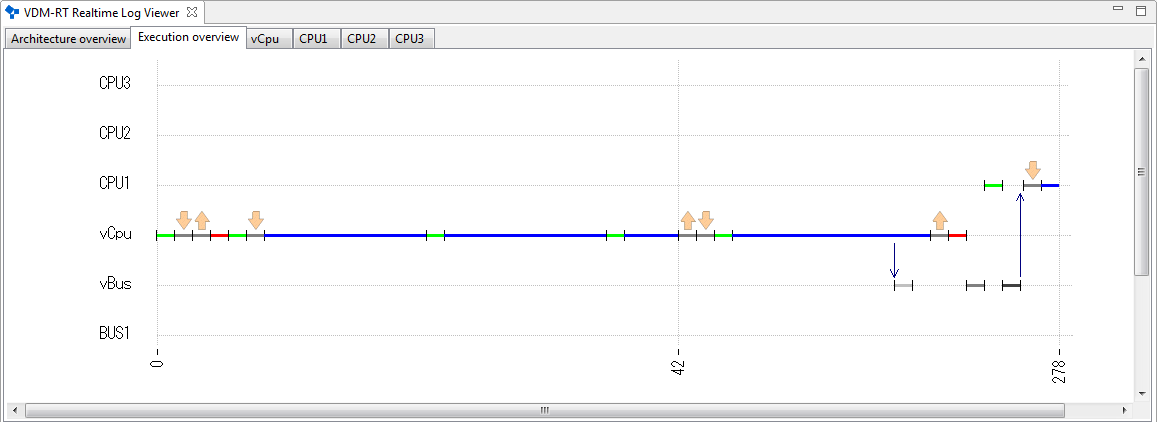
\includegraphics[width=4in]{figures/ExecutionOverview}
  \caption{Execution overview}
  \label{fig:userguide:ExecutionOverview}
\end{center}
\end{figure}

Since the complete execution of a model cannot generally be shown in a normal
sized window, you have the option of jumping to a certain time index
using the \emph{Go to time} button.\index{Go to time} It is
also possible to export all the generated views to JPEG format files
using the \emph{Export Image} button.\index{export image button} All
the generated images will be placed in the same folder as the \texttt{.logrt}
file.

The log viewer can
also give an overview of all executions on a single CPU. This view
gives a detailed description of all operations and functions invoked
on the one CPU as well as the scheduling of concurrent processes. See
Figure~\ref{fig:userguide:ExecutionCPU}.\index{single CPU overview} 

\begin{figure}[htp]
\begin{center}
  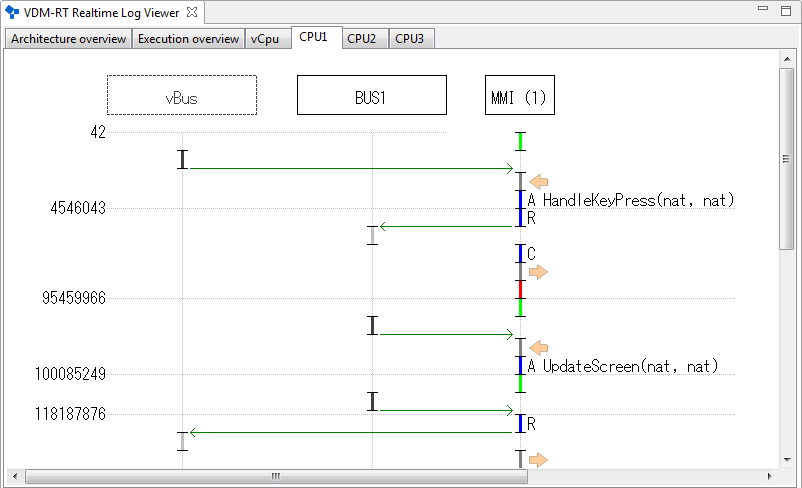
\includegraphics[width=4in]{figures/ExecutionCPU}
  \caption{Execution on single CPU}
  \label{fig:userguide:ExecutionCPU}
\end{center}
\end{figure}

\chapter{Defining Your Own Java Libraries to be used from Overture}\label{sec:javalibs}

VDM models are not appropriate for describing everything. It is common
to have existing legacy code that you may not
wish to spend time modelling in VDM, but would like to make use of
from a VDM model. Overture has a feature to link a VDM
model with external Java libraries contained in a standard \texttt{jar} file
\footnote{In fact the \texttt{IO}, \texttt{MATH}, \texttt{Util},
  \texttt{CSV} and \texttt{VDM-Unit} libraries are implemented as such
external jar files.}.
Using this feature it is possible 
to call functionality provided by jar files from a VDM model. This functionality
corresponds to DL modules/classes in VDMTools\cite{DLMan}.

External jar libraries are linked to VDM via
\texttt{is not yet specified} statements and expressions. Operations
or functions of modules or classes can be delegated to an external
jar, calling out to a Java class. The Java delegate, if present, has
the same name as the VDM
module/class name with underscores (``\_'') replaced with package naming
dots (``.''). For example, the VDM class \texttt{remote\_lib\_sensor} becomes
the class \texttt{remote.lib.sensor} in Java. The delegate lookup is only done once and
only when an \texttt{is not yet specified} statement or expression is first
reached in a class or module. The jar with the external library must be placed in
the VDM project in a subfolder named \texttt{lib} where it will be put in the
class-path of the interpreter when it is executed.

\section{External Library Example}

In this example, a remote sensor will be defined in VDM which can read a
value from a real sensor. The VDM model interface of the sensor can be
seen in listing~\ref{remoteSensorVdm} and the Java class
implementing it can be seen in listing~\ref{remoteSensorJava}. The
values that are to be exchanged between the Overture IDE and the jar
file needs to be the internal \emph{Value} objects used in VDMJ. Documentation about
these classes can be found in the VDMJ Design Specification\cite{Battle10}.

\begin{lstlisting}[language=VDM++,label=remoteSensorVdm,caption=Remote sensor VDM class,captionpos=b]
class remote_lib_sensor

operations

public getValue : int ==> int
getValue (id) == is not yet specified;

end remote_lib_sensor
\end{lstlisting}


\begin{lstlisting}[language=JAVA,label=remoteSensorJava,caption=Remote sensor Java class,captionpos=b]
package remote.lib;

import org.overturetool.vdmj.runtime.ValueException;
import org.overturetool.vdmj.values.IntegerValue;
import org.overturetool.vdmj.values.Value;

public class sensor
{
	public Value getValue(Value id) throws ValueException
	{
		int result = ... // Read a value for sensor number "id"
		return new IntegerValue(result);
	}
}
\end{lstlisting}

\chapter{Enabling Remote Control of the Overture
  Interpreter}\label{sec:remote}

In some situations, it may be valuable to be able to establish a
front end (for example a GUI or a test harness) for calling a VDM model.
This feature corresponds roughly to the CORBA based API from
VDMTools\cite{APIMan}.

A VDM model can be remotely controlled by implementing the Java interface
\texttt{RemoteControl}. Remote control should be understood as a
delegation of control of the interpreter, which means that the remote
controller is in charge of the execution or debug session and is responsible for taking
action and executing parts of the VDM model when needed. When finished, it should
return and the session will stop. When a Remote controller is
used, the Overture debugger continues working normally, so for example
breakpoints can be used in debug mode. A debugging session with the use of a remote
controller can be started by placing the jar with the RemoteControl implementation
in a project subfolder called \texttt{lib}. The fully
qualified name of the RemoteControl class must then be specified in the
launch configuration in the \textit{Remote Control} box.

\section{Example of a Remote Control Class}

In this example, we have a VDM class \texttt{A} which defines an operation
that just returns its argument. As
seen in listing~\ref{remoteControllerJava}, it is possible to call
\texttt{execute} on the Overture interpreter via the RemoteInterpreter object
which is passed to the RemoteControl implementation via the \texttt{run} method.
The method returns a string with the result. A more
advanced \texttt{valueExecute} method is also available which returns the internal
Value type of the interpreter which is useful for more complex
results. The values exchanged between the Overture IDE and the 
controller are the internal Values used in VDMJ. Documentation about these
can be found in the VDMJ Design Specification\cite{Battle10}.

\begin{lstlisting}[language=JAVA,label=remoteControllerJava,caption=Remote Controller Java class,captionpos=b]
import org.overturetool.vdmj.debug.RemoteControl;
import org.overturetool.vdmj.debug.RemoteInterpreter;

public class RemoteController implements RemoteControl
{
	public void run(RemoteInterpreter interpreter) throws Exception
	{
		System.out.println("Remote controller run");
		System.out.println("The answer is " + 
			interpreter.execute("1 + 1")); 
		System.out.println("The answer is " + 
			interpreter.execute("new A().op(123)")); 
		System.out.println("The answer is " + 
			interpreter.execute("new A().op(1 + 3)")); 
	}
}
\end{lstlisting}

\chapter{A Command-Line Interface to VDMJ}\label{sec:commandline}

At the centre of the Overture tool there is a Java implementation of VDM
called \emph{VDMJ}. This provides a command-line interface that may be valuable
as it can be used independently of the Eclipse interface of Overture.
\index{VDMJ}

\section{Starting VDMJ}

VDMJ\index{VDMJ} is contained entirely within one jar file. The jar
file contains a MANIFEST that identifies the main class to start the
tool, so the minimum command line invocation is as follows:

\lstset{style=tool,language=}
\begin{lstlisting}
$ !\textbf{java -jar vdmj-2.0.2.jar}!
VDMJ: You must specify either -vdmsl, -vdmpp or -vdmrt
Usage: VDMJ <-vdmsl | -vdmpp | -vdmrt> [<options>] [<files>]
\end{lstlisting}
\lstset{style=mystyle}
\lstset{language=VDM++}

The first parameter indicates the VDM dialect to use and then
various extra options can be used. These are:

\begin{description}
\item[\texttt{-r}:] This indicates the VDM release number (classic or vdm10).
\item[\texttt{-w}:] This will suppress all warning messages.
\item[\texttt{-q}:] This will suppress all information messages, such as
 the number of source files processed etc.
\item[\texttt{-i}:] This will start the command line interpreter if the VDM
  model is successfully parsed and type checked, otherwise the errors discovered
  will be listed.
\item[\texttt{-p}:] This will generate all proof obligations for the
  VDM model (if it is syntax and type correct) and then stop.
\item[\texttt{-e <exp>}:] This will evaluate the \texttt{<exp>}, print
  the result, and stop.
\item[\texttt{-c <charset>}:] This will select a file character set, to
allow a specification written in languages other than the default for your system. 
\item[\texttt{-t <charset>}:] This will select a console character set. The output
terminal can use a different character set to the specification files.
\item[\texttt{-o <filename>}:] This will save the internal
  representation of a parsed and type checked spe\-ci\-fication. Such files are
  effectively libraries, and can be can be re-loaded without the
  parsing/checking overhead. If files are sufficiently large, this may be faster.
\item[\texttt{-pre}:] This will disable all pre-condition checks.
\item[\texttt{-post}:] This will disable all post-condition checks.
\item[\texttt{-inv}:] This will disable type/state invariant checks.
\item[\texttt{-dtc}:] This will disable all dynamic type checking.
\item[\texttt{-measures}:] This will disable recursive measure checking.
\item[\texttt{-log}:] This will enable VDM-RT real-time event logging (see Chapter~\ref{sec:showlog}).
\item[\texttt{-remote}:] This enables remote control of the VDMJ executable.
\end{description}

Normally, a VDM model will be loaded by identifying all of the VDM source files to include. At least
one source file must be specified unless the -i option is used, in which case the interpreter can be
started with no specification. If a directory is specified rather than a file, then VDMJ will load
all files in that directory with a suffix that matches the dialect (eg. \texttt{*.vdmpp} files for VDM++).
Multiple files and directory arguments can be mixed.

If no \texttt{-i} option is given, the tool will only parse and type check
the VDM model files, giving any errors and warnings on
standard output, then stop. 
%Warnings can be suppressed with the \texttt{-w}
%option. The \texttt{-q} option can be used to suppress the various
%information messages printed (this does not include errors and
%warnings).

The \texttt{-p} option will run the proof obligation generator and
then stop, assuming the specification has no type checking errors.

For batch execution, the \texttt{-e} option can be used to identify a
single expression to evaluate in the context of the loaded
specification, assuming the specification has no type checking errors.

%The \texttt{-c} and \texttt{-t} options allow the file and console character sets to be defined, respectively. 

%The \texttt{-o} option allows a parsed and type checked specification to be saved to a file.
%The \texttt{-pre}, \texttt{-post}, \texttt{-inv} and \texttt{-dtc} options can be used to disable precondition, postcondition, invariant and
%dynamic type checking, respectively. By default, all these checks are performed.
%The \texttt{-log} option is for use with \texttt{-vdmrt}, and causes real-time events from the model to be written to the
%file name given. 

%If flat.vdmsl contains a simple VDM-SL specification of the factorial
%function, called ``\texttt{fac}'', the following
%illustrate ways to test the specification, with user input shown in bold:

%\begin{lstlisting}
%functions
%fac: int -> int
%fac(a) == if a < 2 then 1 else a * fac(a-1)
%pre a > 0
%\end{lstlisting}
\lstset{style=tool,language=}

%\begin{lstlisting}
%$ !\textbf{java -jar vdmj-2.0.0.jar -vdmsl flat.vdmsl}!
%Parsed 1 module in 0.202 secs. No syntax errors
%Warning 5012: Recursive function has no measure in (flat.vdmsl) at 
%line 3:1
%Type checked 1 module in 0.016 secs. No type errors and 1 warning
%\end{lstlisting}

%\begin{lstlisting}
%$ !\textbf{java -jar vdmj-2.0.0.jar -vdmsl -q -w flat.vdmsl}!
%<quiet>
%\end{lstlisting}

%\begin{lstlisting}
%$ !\textbf{java -jar vdmj-2.0.0.jar -vdmsl -w -e "fac(10)" flat.vdmsl}!
%Parsed 1 module in 0.28 secs. No syntax errors
%Type checked 1 module in 0.031 secs. No type errors, 
%suppressed 1 warning
%Initialized 1 module in 0.031 secs.
%3628800
%Bye
%\end{lstlisting}

%\begin{lstlisting}
%$ !\textbf{java -jar vdmj-2.0.0.jar -vdmsl -e "fac(10)" -q -w flat.vdmsl}!
%3628800
%\end{lstlisting}

%\begin{lstlisting}
%$ !\textbf{java -jar vdmj-2.0.0.jar -vdmsl -i -w flat.vdmsl}!
%Parsed 1 module in 0.202 secs. No syntax errors
%Type checked 1 module in 0.016 secs. No type errors, 
%suppressed 1 warning
%Initialized 1 module in 0.031 secs.
%Interpreter started
%> !\textbf{print fac(10)}!
%= 3628800
%Executed in 0.0 secs.
%> !\textbf{quit}!
%Bye
%\end{lstlisting}

%\begin{lstlisting}
%$ !\textbf{java -jar vdmj-2.0.0.jar -vdmsl -p -w flat.vdmsl}!
%Parsed 1 module in 0.218 secs. No syntax errors
%Type checked 1 module in 0.015 secs. No type errors, 
%suppressed 1 warning
%Generated 1 proof obligation:
%Proof Obligation 1:
%fac: function apply obligation in 'DEFAULT1' (flat.vdmsl) at 
%line 4:38
%(forall a:int & (a > 0) =>
%(not (a < 2) =>
%pre_f((a - 1))))
%\end{lstlisting}

%\begin{lstlisting}
%$ !\textbf{java -jar vdmj-2.0.0.jar -vdmsl -w -e "fac(0)" -w flat.vdmsl}!
%Parsed 1 module in 0.203 secs. No syntax errors
%Type checked 1 module in 0.015 secs. No type errors, 
%suppressed 1 warning
%Initialized 1 module in 0.016 secs.
%Execution: Error 4055: Precondition failure: pre_f in (flat.vdmsl) 
%at line 5:11
%   a = 0
%   fac = (int -> int)
%   pre_fac = (int +> bool)
%In root context of fac(a) in 'DEFAULT1' (console) at line 1:1
%In root context of interpreter in 'DEFAULT1' (flat.vdmsl) at 
%line 3:1
%In root context of global environment
%Bye
%\end{lstlisting}

%\begin{lstlisting}
%$ !\textbf{java -jar vdmj-2.0.0.jar -vdmsl -w -pre -e "fac(0)" 
%-w flat.vdmsl}!
%Parsed 1 module in 0.218 secs. No syntax errors
%Type checked 1 module in 0.016 secs. No type errors, 
%suppressed 1 warning
%Initialized 1 module in 0.015 secs.
%1
%Bye
%\end{lstlisting}

%\begin{lstlisting}
%$ !\textbf{java -jar vdmj-2.0.0.jar -vdmsl -w -o flat.lib flat.vdmsl}!
%Parsed 1 module in 0.203 secs. No syntax errors
%Type checked 1 module in 0.016 secs. No type errors, 
%suppressed 1 warning
%Saved 1 module to flat.lib in 0.093 secs.
%\end{lstlisting}

%\begin{lstlisting}
%$ !\textbf{java -jar vdmj-2.0.0.jar -vdmsl flat.lib -e "fac(10)"}!
%Loaded 1 module from flat.lib in 0.187 secs
%Initialized 1 module in 0.0 secs.
%3628800
%Bye
%\end{lstlisting}

\section{Parsing, Type Checking, and Proof Obligations in VDMJ}

All specification files loaded by VDMJ are parsed and type checked
automatically. There are no type checking options; the type checker
always uses \texttt{possible} semantics. If a specification does not parse
and type check cleanly, the interpreter cannot be started and proof
obligations cannot be generated (though warnings are allowed). All
warnings and error messages are printed on standard output, even
with the \texttt{-q} option.

A source file may contain VDM definitions embedded
in a \LaTeX\ file using \verb|vdm_al| environments (see
Chapter~\ref{sec:prettyprint}); the markup is ignored by the parser,
though reported line numbers will be correct. Note that each source file
must start with a recognizable \LaTeX\ construct:
a \verb+\documentclass, \section, \subsection+ or a \LaTeX\ comment.

The VDMJ Java process will return with an exit code of zero if the
specification is clean (ignoring warnings). Parser or type checking
errors result in an exit code of 1. The interpreter and PO generator
always exit with a code of zero.

\section{The VDMJ Interpreter and Debugger}\label{sec:commandlineinterpreter}

Assuming a specification does not contain any parse or type checking errors, the interpreter can be
started by using the \texttt{-i} command line option.
The interpreter is an interactive command line tool that allows expressions to be evaluated in the
context of the specification loaded. For example, to load and interpret a
VDM-SL specification from a single file called \texttt{shmem.vdmsl},
the following options would be used:

\begin{lstlisting}
$ !\textbf{java -jar vdmj-2.0.2.jar -vdmsl -i shmem.vdmsl}!
Parsed 1 module in 0.266 secs. No syntax errors
Type checked in 0.047 secs. No type errors
Interpreter started
\end{lstlisting}

The interpreter prompt is ``\texttt{>}''. The 
interactive interpreter commands are as follows (abbreviated forms are
permitted for some, shown in square brackets): 
% (explanation below. The shmem.vdmsl source
%model is in Appendix A):

\begin{description}
\item[\texttt{modules}:] This command lists the loaded module names in
  a VDM-SL specification. For a flat VDM-SL model, the single name
  \texttt{DEFAULT} is used. The default module will be indicated in
  the list displayed.\index{modules}\index{command!modules}
\item[\texttt{classes}:] This command lists the loaded class names in
  VDM++ and VDM-RT specifications. The default class will be indicated in
  the list displayed.\index{classes}\index{command!classes}
\item[\texttt{default <module/class>}:] This command sets the default
  module/class name as the prime scope for which the lookup of
  identifiers appear (i.e.\ names in the default module
  do not need to be qualified, so you can say ``\texttt{print xyz}'' rather than
``\texttt{print M`xyz}'').\index{default}\index{command!default}
\item[\texttt{create <id> := <exp>}:] This command is only available
  for the VDM++ and VDM-RT dialects. It creates a global variable that
  can be used subsequently in the interpreter. It is mostly used for
  creating global instances of classes.\index{create}\index{command!create} 
\item[\texttt{log [<file> | off]}:] This command can only be used with
  VDM-RT models. It starts to log real-time events to the file indicated. By
  default, event logging is turned off. Logging can be directed to
  the console by using log with no arguments, or to a file using \texttt{log
  <filename>}. Logging can subsequently be turned off again by using
  \texttt{log off}. The events logged include requests, activations and
  completions of all functions and operations, as well as all object creations,
  creation of CPUs and BUSses, deployment of objects
  to specific CPUs and the swapping in/out of threads.\index{log}\index{command!log}  
\item[\texttt{state}:] This command can only be used for the VDM-SL
  dialect and shows the default module state.\index{state}\index{command!state}  
  The value of the state can be changed by operations called.
\item[\texttt{[p]rint <expression>}:] This command evaluates the
  expression provided in the current context.\index{print}\index{command!print}     
\item[\texttt{runtrace <name> [test number]}:] This command runs the trace called
  \texttt{<name>}. This will expand the combinatorial
  test and execute the resulting
  operation sequences. If a specific test number is provided, only
  that one test from the expansion will be executed. \index{combinatorial testing}
\item[\texttt{debugtrace <name> [test number]}:] This command is the same as
  \texttt{runtrace}, except that if a runtime exception is encountered during
  the execution of a test, control will enter the debugger. With \texttt{runtrace},
  runtime exceptions are recorded as the result of a (failed) test, rather than
  trapping into the debugger.\index{combinatorial testing}
\item[\texttt{filter \%age | <reduction type>}:] This command reduces
  the size of expanded CT traces to a given percentage (eg. 10\%).
  There are various options for making the actual selection of tests to remove:
  ``\texttt{RANDOM}'', ``\texttt{SHAPES\_NOVARS}'', ``\texttt{SHAPES\_VARNAMES}''
   or ``\texttt{SHAPES\_VARVALUES}'' (the names are not case sensitive).
\item[\texttt{assert <file>}:] This command runs assertions from the
  file provided. The assertions in the file must be Boolean
  expressions, one per line. The command evaluates every assertion in
  the file, raising an error for any which is false.\index{assert}\index{command!assert}  
\item[\texttt{init}:] This command re-initializes the global
  environment. Thus all state components will be initialised to their
  initial value again, created variables are lost and code coverage information
  is reset.\index{init}\index{command!init} 
\item[\texttt{env}:] This command lists the value of all global symbols
  in the default environment. This will show the signatures for all
  functions and operations as well as the values assigned to
  identifiers from value definitions and global state definitions (in VDM++
  terminology, public static instance variables). Note that this includes invariant,
  initialization and pre/postcondition functions. In the VDM++ and
  VDM-RT dialects, the identifiers created using the \texttt{create}
  command will also be included.\index{env}\index{command!env} 
\item[\texttt{pog [<fn/op>]}:] This command generates a list of all proof
  obligations for the VDM model that is loaded. There is an optional argument
  to indicate one function or operation name.\index{pog}\index{command!pog}  
\item[\texttt{break [<file>:]<line\#> [<condition>]}:] This command
  creates a breakpoint at a specific file and line and optionally makes
  it a conditional breakpoint.\index{break}\index{command!break}  
\item[\texttt{break <function/operation> [<condition>]}:] This command
  creates a breakpoint at the start of the body of a named function or operation and
  optionally makes it a conditional breakpoint. 
\item[\texttt{trace [<file>:]<line\#> [<exp>]}:] This command creates a
  tracepoint for a specific file and line. A tracepoint prints the value of the
  expression given whenever the tracepoint is reached, and then continues.
  \index{trace}\index{command!trace} 
\item[\texttt{trace <function/operation> [<exp>]}:] This command
  create a tracepoint at the start of a function or operation body.
  See \texttt{trace} above for an explanation of tracepoints.
\item[\texttt{remove <breakpoint\#>}:] This command removes a
  trace/breakpoint by referring to its number (given by the
  \texttt{list} command).\index{remove}\index{command!remove} 
\item[\texttt{list}:] This command provides a list of all current
  trace/breakpoints by number.\index{list}\index{command!list}  
\item[\texttt{coverage [clear|write <dir>|merge <dir>|<filenames>]}:]
  This command manages test coverage information.
  The coverage command displays the source
  code of the loaded VDM model (by default, all source files are
  listed), with ``+'' and ``-'' signs in the left hand column
  indicating lines which have been executed or not. The percentage
  coverage of each source file
  is displayed.\index{coverage}\index{command!coverage} Typically, the
  testing of a specification will be incremental, and so it is
  convenient to be able to ``save'' the coverage achieved in each test
  session, and subsequently merge the results together. This can be
  achieved with the \texttt{write <dir>} and \texttt{merge <dir>} options to the
  coverage command. The write option saves the current coverage
  information in \texttt{<dir>} for each specification file loaded; the merge
  option reads this information back, and merges it with the current
  coverage information. For example, each day's test coverage could be
  written to a separate ``day'' directory, and then all the days merged
  together for review of the overall coverage at the end.
\item[\texttt{latex|latexdoc [<files>]}:] This command generates \LaTeX\
  coverage files. These are \LaTeX\ versions of the source files
  with parts of the
  specification highlighted where they have not been executed. The
  \LaTeX\ output also contains a table of percentage cover by
  module/class and the number of times functions and operations were
  hit during the execution. The \texttt{latexdoc} command is the same,
  except that output files are wrapped in \LaTeX\ document headers. The
  output files are written to the same directory as the source files, one
  per source file, with the extension \texttt{.tex}. Coverage
  information is reset when a specification is loaded, when an \texttt{init}
  command is given, or when the
  command \texttt{coverage clear} is executed, otherwise coverage is
  cumulative. If several files are loaded, the coverage for just one
  source file can be listed with \texttt{coverage <file>} or
  \texttt{latex <file>}. \index{latex}\index{command!latex} 
  \index{latexdoc}\index{command!latexdoc} 
\item[\texttt{files}:] This command lists the names of all source files loaded.
  \index{files}\index{command!files} 
\item[\texttt{reload}:] This command will reload, parse and type check the
  VDM model files currently loaded. Note that if there are any errors
  in the parse or type check of the files, the interpreter will exit
  after the reload.\index{reload}\index{command!reload} 
\item[\texttt{load <files>}:] This command replaces the current loaded VDM
  model files. Note that if there are any errors in the parse or type
  check of the files, the interpreter will exit after
  the load.\index{load}\index{command!load}  
\item[\texttt{[q]uit}:] This command leaves the
  interpreter.\index{quit}\index{command!quit}  
\end{description}

%\begin{lstlisting}
%> !\textbf{modules}!
%M (default)
%\end{lstlisting}

%\begin{lstlisting}
%> !\textbf{state}!
%M`Q4 = [mk_M(<FREE>, 0, 9999)]
%M`rseed = 87654321
%M`Memory = mk_Memory(87654321, [mk_M(<FREE>, 0, 9999)],
%                               [mk_M(<FREE>, 0, 9999)])
%M`Q3 = [mk_M(<FREE>, 0, 9999)]
%\end{lstlisting}

%\begin{lstlisting}
%> !\textbf{print rand(100)}!
%= 71
%Executed in 0.0 secs.
%\end{lstlisting}

%\begin{lstlisting}
%> !\textbf{print rand(100)}!
%= 44
%Executed in 0.0 secs.
%\end{lstlisting}

%\begin{lstlisting}
%> !\textbf{state}!
%M`Q4 = [mk_M(<FREE>, 0, 9999)]
%M`rseed = 566044643
%M`Memory = mk_Memory(566044643, [mk_M(<FREE>, 0, 9999)], 
%                                [mk_M(<FREE>, 0, 9999)])
%M`Q3 = [mk_M(<FREE>, 0, 9999)]
%\end{lstlisting}

%\begin{lstlisting}
%> !\textbf{init}!
%Global context initialized
%\end{lstlisting}

%\begin{lstlisting}
%> !\textbf{state}!
%M`Q4 = [mk_M(<FREE>, 0, 9999)]
%M`rseed = 87654321
%M`Memory = mk_Memory(87654321, [mk_M(<FREE>, 0, 9999)],
%                               [mk_M(<FREE>, 0, 9999)])
%M`Q3 = [mk_M(<FREE>, 0, 9999)]
%\end{lstlisting}

%\begin{lstlisting}
%> !\textbf{print rand(100)}!
%= 71
%Executed in 0.0 secs.
%\end{lstlisting}

%\begin{lstlisting}
%> !\textbf{print rand(100)}!
%= 44
%Executed in 0.0 secs.
%\end{lstlisting}

%\begin{lstlisting}
%> !\textbf{env}!
%M`fragments = (M`Quadrant -> nat)
%M`combine = (M`Quadrant -> M`Quadrant)
%M`tryBest = (nat ==> nat)
%M`seed = (nat1 ==> ())
%M`reset = (() ==> ())
%M`bestfit = (nat1 * M`Quadrant -> nat1)
%M`add = (nat1 * nat1 * M`Quadrant -> M`Quadrant)
%M`firstFit = (nat1 ==> bool)
%M`rand = (nat1 ==> nat1)
%M`tryFirst = (nat ==> nat)
%M`main = (nat1 * nat1 ==> seq of (<SAME> | <BEST> | <FIRST>))
%M`MAXMEM = 10000
%M`delete = (M`M * M`Quadrant -> M`Quadrant)
%M`inv_M = (M`M +> bool)
%M`CHUNK = 100
%M`bestFit = (nat1 ==> bool)
%M`least = (nat1 * nat1 -> nat1)
%M`fits = (nat1 * M`Quadrant -> nat1)
%M`init_Memory = (M`Memory +> bool)
%M`pre_add = (nat1 * nat1 * M`Quadrant +> bool)
%\end{lstlisting}

%\begin{lstlisting}
%> !\textbf{pog}!
%Generated 36 proof obligations:
%Proof Obligation 1:
%M`fits: cases exhaustive obligation in 'M' (shmem.vdm) at 
%line 40:5
%(forall size:nat1, Q:Quadrant &
%Q = [] or Q = [h] ^ tail)
%...
%Proof Obligation 35:
%M`tryBest: sequence apply obligation in 'M' (shmem.vdm) at 
%line 176:27
%rand((len Q4)) in set inds Q4
%Proof Obligation 36:
%M`tryBest: subtype obligation in 'M' (shmem.vdm) at line 166:1
%RESULT >= 0
%\end{lstlisting}

%This example shows a VDM-SL specification called \texttt{shmem.vdmsl} being
%loaded. The help command lists the interpreter commands
%available. Note that several of them regard the setting of
%breakpoints, which is covered in the next section.

%The modules command lists the names of the modules loaded from the
%specification. In this example there is only one, called ``M''. One of
%the modules is identified as the default; names in the default module
%do not need to be qualified (so you can say print xyz rather than
%print M`xyz). The default module can be changed with the default
%command.

%The state command lists the content of the default module's
%state. This can be changed by operations, as can be seen by the two
%calls to rand which change the rseed value in the state (a
%pseudo-random number generator). The {\ttfamily{\bf init}} command will re-initialize
%the state to its original value, illustrated by the fact that two
%subsequent calls to rand return the same results as the first two did.

%The {\ttfamily{\bf print}}\index{print} command can be used to
%evaluate any expression.  The {\ttfamily{\bf env}}\index{env} command
%lists all the values in the global environment of the default
%module. This shows the functions, operations and constant values
%defined in the module. Note that it includes invariant, initialization
%and pre/postcondition functions.  The {\ttfamily{\bf pog}} command (proof obligation
%generator) generates a list of proof obligations for the
%specification.

%The assert command\index{assert} (illustrated below) can take a list of assertions
%from a file, and execute each of them in turn, raising an error for
%any assertion which is false. The assertions in the file must be
%simple boolean expressions, one per line:

When the execution of a VDM model is stopped at a
breakpoint, there are additional commands that can be used. These are:

\begin{description}
\item[\texttt{[s]tep}:] This command steps forward until the
  current expression/statement is on a new line. The command will step
  into function and operation calls.\index{step}\index{command!step} 
\item[\texttt{[n]ext}:] This command is similar to \texttt{step} except
 function and operation calls are stepped over.\index{next}\index{command!next}  
\item[\texttt{[o]ut}:] This command runs to the return of the current
  function or operation.\index{out}\index{command!out} 
\item[\texttt{[c]ontinue}:] This command resumes execution and continues
  until the next breakpoint or completion of the thread that is being
  debugged.\index{continue}\index{command!continue} 
\item[\texttt{stack}:] This command displays the current stack frame
  context (i.e.\ the call stack).\index{stack}\index{command!stack} 
\item[\texttt{up}:] This command moves the stack frame context up one
  frame to allow variables to be seen.\index{up}\index{command!up}  
\item[\texttt{down}:] This command moves the stack frame context down
  one frame.\index{down}\index{command!down}  
\item[\texttt{source}:] This command lists VDM source around the
  current breakpoint. \index{source}\index{command!source} 
\item[\texttt{stop}:] This command terminates the execution
  immediately.\index{stop}\index{command!stop}  
\item[\texttt{threads}:] This command can only be used for the VDM++
  and VDM-RT dialects. It lists the active threads with status
  information for each thread.\index{threads}\index{command!threads} 
\end{description}

\appendix
\newpage

\bibliographystyle{nnewalpha}

\bibliography{bib/UserGuide,dan}
\addcontentsline{toc}{section}{\protect\numberline{}{References}}

\newpage
\chapter{Templates in Overture}\label{app:templates}

Overture defines a number of standard Eclipse templates. You can add
your own as well. The keys and descriptions of the pre-defined templates
are:

\begin{longtable}{| l| p{9cm}| }\hline
Key & Description\\\hline
% ALL 
caseExpression            & Case Expression\\
dclStatement              & Declare\\
defExpression             & def pattern = expression1 in expression2\\
exists                    & exists bindList \& predicate\\
forall                    & forall bind list \& predicate\\
forallLoop                & for identifier = expression1 to expression2 do statement\\
forallinset               & forall in set\\
functions                 & Function block\\
ifthen                    & if predicate then expression1 else expression2\\
let                       & let pattern = expression1 in expression2\\
operations                & Operation block\\
while                     & while predicate do statement\\

% VDM-SL 
functionExplicit          & Explicit function\\
functionImplicit          & Implicit function\\
module                    & Module\\
moduleSkeleton            & Module Full skeleton of a module\\
operationExplicit         & Explicit Operation\\
operationImplicit         & Implicit operation\\

% VDM-PP 
act                       & The number of times that operation name operation has been activated\\
active                    & The number of operation name operations that are currently active.\\
class                     & Class Definition\\
classSkeleton             & Class Definition full skeleton\\
fin                       & The number of times that the operation name operation has been completed\\
functionExplicit          & Explicit function\\
functionImplicit          & Implicit function\\
instancevariables         & Instance Variables block\\
isnotyetspecified         & is not yet specified\\
isofbaseclass             & Test if an object is of a specific base class\\
isofclass                 & Test if an object is of class\\
issubclassof              & Is subclass of\\
issubclassresponsibility  & Is subclass responsibility\\
mutex                     & Mutex operation\\
operationExplicit         & Explicit Operation\\
operationImplicit         & Implicit operation\\
per                       & Permission predicate for an operation, history counters can be used: \#fin, \#act, \#active, \#req, \#waiting\\
req                       & The number of requests that has been issued for the operation name operation\\
samebaseclass             & Test if two objects are of the same type\\
self                      & Get a reference to the current object\\
sync                      & Synchronization block\\
values                    & Values block\\
waiting                   & The number of outstanding requests for the operation name operation\\

% VDM-RT 
act                       & The number of times that operation name operation has been activated\\
active                    & The number of operation name operations that are currently active.\\
bus                       & BUS (Priority $<$CSMACD$>$, capacity,set of connected CPUs)\\
class                     & Class Definition\\
classSkeleton             & Class Definition full skeleton\\
cpu                       & CPU (Priority $<$FP/FCFS$>$, capacity)\\
cycle                     & Cycles (number of cycles) statement\\
duration                  & Duration (time in nanoseconds) statement\\
fin                       & The number of times that the operation name operation has been completed\\
functionExplicit          & Explicit function\\
functionImplicit          & Implicit function\\
instancevariables         & Instance Variables block\\
isnotyetspecified         & is not yet specified\\
isofbaseclass             & Test if an object is of a specific base class\\
isofclass                 & Test if an object is of class\\
issubclassof              & Is subclass of\\
issubclassresponsibility  & Is subclass responsibility\\
mutex                     & Mutex operation\\
operationExplicit         & Explicit Operation\\
operationImplicit         & Implicit operation\\
per                       & Permission predicate for an operation, history counters can be used: \#fin, \#act, \#active, \#req, \#waiting\\
periodic                  & periodic(periode,jitter,delay,offset)(operation name)\\
req                       & The number of requests that has been issued for the operation name operation\\
samebaseclass             & Test if two objects are of the same type\\
self                      & Get a reference to the current object\\
sync                      & Synchronization block\\
system                    & System skeleton\\
time                      & Get the current time\\
values                    & Values block\\
waiting                   & The number of outstanding requests for the operation name operation\\\hline
\end{longtable}

\newpage
\chapter{Internal Errors}\label{app:internalerrors}

This appendix gives a list of the internal errors in Overture
and the circumstances under which each internal error can be expected.
Most of these errors should \emph{never} be seen, so if they appear
please report the occurrence via the Overture bug reporting utility
(\url{https://sourceforge.net/tracker/?group_id=141350&atid=749152}). 

% VDMJ Error and Warning Messages
% ===============================
%
% Messages and warnings are numbered in the following blocks:
%
% 0000-0999	Internal errors
% 1000-1999	Lexical errors
% 2000-2999	Syntax errors
% 3000-3999	Type checking errors
% 4000-4999	Runtime errors
% 5000-5999	Warnings
%
% Several messages appear to be duplicates, but internally they are raised from
% different places in the code, and so the exact error number may be used to
% distinguish the cases. Some errors are followed by additional detail, such
% as the expected and actual values.

\begin{description}
\item[0000:] \texttt{File IO errors, eg. "File not found"}  This
  typically occurs if a specification file is no longer present.
\item[0001:] \texttt{"Mark/reset not supported - use push/pop"}
\item[0002:] \texttt{"Cannot change type qualifier:\ <name><qualifiers> to <qualifiers>"}
\item[0003:] \texttt{"PatternBind passed <class name>"}
\item[0004:] \texttt{"Cannot get bind values for type <type>"}
\item[0005:] \texttt{"Illegal clone"}
\item[0006:] \texttt{"Constructor for <class> can't find <member>"}
\item[0007:] \texttt{"Cannot write to IO file <name>"}
\item[0009:] \texttt{"Too many syntax errors"}  This error typically
  occurs if one have included a file that is in a non VDM format and
  by mistake have given it a vdm file extension (\texttt{vdmsl},
  \texttt{vdmpp} or \texttt{vdmrt}).\index{vdm file extension}
\item[0010:] \texttt{"Too many type checking errors"}
\item[0011:] \texttt{"CPU or BUS creation failure"}
\item[0052:] \texttt{"Cannot set default name at breakpoint"}
\item[0053:] \texttt{"Unknown trace reduction type"}
\item[0054:] \texttt{"Cannot instantiate native object:\ <reason>"}
\item[0055:] \texttt{"Cannot access native object:\ <reason>"}
\item[0056:] \texttt{"Native method cannot use pattern arguments:\ <sig>"}
\item[0057:] \texttt{"Native member not found:\ <name>"}
\item[0058:] \texttt{"Native method does not return Value:\ "}
\item[0059:] \texttt{"Failed in native method:\ <reason>"}
\item[0060:] \texttt{"Cannot access native method:\ <reason>"}
\item[0061:] \texttt{"Cannot find native method:\ <reason>"}
\item[0062:] \texttt{"Cannot invoke native method:\ <reason>"}
\item[0063:] \texttt{"No delegate class found:\ <name>"}
\item[0064:] \texttt{"Native method should be static:\ <name>"}
\item[0065:] \texttt{"Illegal Lock state"}
\item[0066:] \texttt{"Thread is not running on a CPU"}
\item[0067:] \texttt{"Exported type <name> not structured"}
\item[0068:] \texttt{"Periodic threads overlapping"}
\end{description}


\newpage
\chapter{Lexical Errors}\label{app:lexerr}

When a VDM model is parsed, the first phase is to gather the single
characters into tokens that can be used in the further
processing. This is called a lexical analysis and errors in this area
can be as follows:

% VDMJ Error and Warning Messages
% ===============================
%
% Messages and warnings are numbered in the following blocks:
%
% 0000-0999	Internal errors
% 1000-1999	Lexical errors
% 2000-2999	Syntax errors
% 3000-3999	Type checking errors
% 4000-4999	Runtime errors
% 5000-5999	Warnings
%
% Several messages appear to be duplicates, but internally they are raised from
% different places in the code, and so the exact error number may be used to
% distinguish the cases. Some errors are followed by additional detail, such
% as the expected and actual values.

\begin{description}
\item[1000:] \texttt{"Malformed quoted character"}
\item[1001:] \texttt{"Invalid char <ch> in base <n> number"}
\item[1002:] \texttt{"Expecting '|->'"}
\item[1003:] \texttt{"Expecting '...'"}
\item[1004:] \texttt{"Expecting '<-:'"}
\item[1005:] \texttt{"Expecting close double quote"}
\item[1006:] \texttt{"Expecting close quote after character"}
\item[1007:] \texttt{"Unexpected tag after '\#'"}
\item[1008:] \texttt{"Malformed module`name"}
\item[1009:] \texttt{"Unexpected character 'c'"}
\item[1010:] \texttt{"Expecting <digits>[.<digits>][e<+-><digits>]"}
\item[1011:] \texttt{"Unterminated block comment"}
\end{description}


\newpage
\chapter{Syntax Errors}\label{app:synerr}

If the syntax of the file you have provided does not meet the
syntax rules for the VDM dialect you wish to use, syntax errors will be
reported. These can be as follows:

% VDMJ Error and Warning Messages
% ===============================
%
% Messages and warnings are numbered in the following blocks:
%
% 0000-0999	Internal errors
% 1000-1999	Lexical errors
% 2000-2999	Syntax errors
% 3000-3999	Type checking errors
% 4000-4999	Runtime errors
% 5000-5999	Warnings
%
% Several messages appear to be duplicates, but internally they are raised from
% different places in the code, and so the exact error number may be used to
% distinguish the cases. Some errors are followed by additional detail, such
% as the expected and actual values.

\begin{description}
\item[2000:] \texttt{"Expecting 'in set' after pattern in set binding"}
\item[2001:] \texttt{"Expecting 'in set' in set bind"}
\item[2002:] \texttt{"Expecting ':' in type bind"}
\item[2003:] \texttt{"Expecting 'in set' after pattern in binding"}
\item[2004:] \texttt{"Expecting 'in set' or ':' after patterns"}
\item[2005:] \texttt{"Expecting list of 'class' or 'system' definitions"}
\item[2006:] \texttt{"Found tokens after class definitions"}
\item[2007:] \texttt{"Expecting 'end <class>'"}
\item[2008:] \texttt{"Class does not start with 'class'"}
\item[2009:] \texttt{"Can't have instance variables in VDM-SL"}
\item[2010:] \texttt{"Can't have a thread clause in VDM-SL"}
\item[2011:] \texttt{"Only one thread clause permitted per class"}
\item[2012:] \texttt{"Can't have a sync clause in VDM-SL"}
\item[2013:] \texttt{"Expected 'operations', 'state', 'functions', 'types' or 'values'"}
\item[2014:] \texttt{"Recursive type declaration"}  This is reported in
  type definitions such as \texttt{T = T}.
\item[2015:] \texttt{"Expecting =<type> or ::<field list>"}
\item[2016:] \texttt{"Function name cannot start with 'mk\_'"}
\item[2017:] \texttt{"Expecting ':' or '(' after name in function definition"}
\item[2018:] \texttt{"Function type is not a -> or +> function"}
\item[2019:] \texttt{"Expecting identifier <name> after type in definition"}
\item[2020:] \texttt{"Expecting '(' after function name"}
\item[2021:] \texttt{"Expecting ':' or '(' after name in operation definition"}
\item[2022:] \texttt{"Expecting name <name> after type in definition"}
\item[2023:] \texttt{"Expecting '(' after operation name"}
\item[2024:] \texttt{"Expecting external declarations after 'ext'"}
\item[2025:] \texttt{"Expecting <name>:\ exp->exp in errs clause"}
\item[2026:] \texttt{"Expecting 'rd' or 'wr' after 'ext'"}
\item[2027:] \texttt{"-"}
\item[2028:] \texttt{"Expecting 'per' or 'mutex'"}
\item[2029:] \texttt{"Expecting <set bind> = <expression>"}
\item[2030:] \texttt{"Expecting simple field identifier"}
\item[2031:] \texttt{"Expecting field number after .\#"}
\item[2032:] \texttt{"Expecting field name"}
\item[2033:] \texttt{"Expected 'is not specified' or 'is subclass responsibility'"}
\item[2034:] \texttt{"Unexpected token in expression"}
\item[2035:] \texttt{"Tuple must have >1 argument"}
\item[2036:] \texttt{"Expecting mk\_<type>"}
\item[2037:] \texttt{"Malformed mk\_<type> name <name>"}
\item[2038:] \texttt{"Expecting is\_<type>"}
\item[2039:] \texttt{"Expecting maplet in map enumeration"}
\item[2040:] \texttt{"Expecting 'else' in 'if' expression"}
\item[2041:] \texttt{"Expecting two arguments for 'isofbase'"}
\item[2042:] \texttt{"Expecting (<class>,<exp>) arguments for 'isofbase'"}
\item[2043:] \texttt{"Expecting two arguments for 'isofclass'"}
\item[2044:] \texttt{"Expecting (<class>,<exp>) arguments for 'isofclass'"}
\item[2045:] \texttt{"Expecting two expressions in 'samebaseclass'"}
\item[2046:] \texttt{"Expecting two expressions in 'sameclass'"}
\item[2047:] \texttt{"Can't use history expression here"}
\item[2048:] \texttt{"Expecting \#act, \#active, \#fin, \#req or \#waiting"}
\item[2049:] \texttt{"Expecting 'end <module>'"}
\item[2050:] \texttt{"Expecting library name after 'uselib'"}
\item[2051:] \texttt{"Expecting 'end <module>'"}
\item[2052:] \texttt{"Expecting 'all', 'types', 'values', 'functions' or 'operations'"}
\item[2053:] \texttt{"Exported function is not a function type"}
\item[2054:] \texttt{"Expecting types, values, functions or operations"}
\item[2055:] \texttt{"Imported function is not a function type"}
\item[2056:] \texttt{"Cannot use module'id name in patterns"}
\item[2057:] \texttt{"Unexpected token in pattern"}
\item[2058:] \texttt{"Expecting identifier"}
\item[2059:] \texttt{"Expecting a name"}
\item[2060:] \texttt{"Found qualified name <name>. Expecting an identifier"}
\item[2061:] \texttt{"Expecting a name"}
\item[2062:] \texttt{"Expected 'is not specified' or 'is subclass responsibility'"}
\item[2063:] \texttt{"Unexpected token in statement"}
\item[2064:] \texttt{"Expecting <object>.identifier(args) or name(args)"}
\item[2065:] \texttt{"Expecting <object>.name(args) or name(args)"}
\item[2066:] \texttt{"Expecting object field name"}
\item[2067:] \texttt{"Expecting 'self', 'new' or name in object designator"}
\item[2068:] \texttt{"Expecting field identifier"}
\item[2069:] \texttt{"Expecting <identifier>:<type> := <expression>"}
\item[2070:] \texttt{"Function type cannot return void type"}
\item[2071:] \texttt{"Expecting field identifier before ':'"}
\item[2072:] \texttt{"Expecting field name before ':-'"}
\item[2073:] \texttt{"Duplicate field names in record type"}
\item[2074:] \texttt{"Unexpected token in type expression"}
\item[2075:] \texttt{"Expecting 'is subclass of'"}
\item[2076:] \texttt{"Expecting 'is subclass of'"}
\item[2077:] \texttt{"Expecting 'end' after class members"}
\item[2078:] \texttt{"Missing ';' after type definition"}
\item[2079:] \texttt{"Missing ';' after function definition"}
\item[2080:] \texttt{"Missing ';' after state definition"}
\item[2081:] \texttt{"Missing ';' after value definition"}
\item[2082:] \texttt{"Missing ';' after operation definition"}
\item[2083:] \texttt{"Expecting 'instance variables'"}
\item[2084:] \texttt{"Missing ';' after instance variable definition"}
\item[2085:] \texttt{"Missing ';' after thread definition"}
\item[2086:] \texttt{"Missing ';' after sync definition"}
\item[2087:] \texttt{"Expecting '==' after pattern in invariant"}
\item[2088:] \texttt{"Expecting '@' before type parameter"}
\item[2089:] \texttt{"Expecting '@' before type parameter"}
\item[2090:] \texttt{"Expecting ']' after type parameters"}
\item[2091:] \texttt{"Expecting ')' after function parameters"}
\item[2092:] \texttt{"Expecting '==' after parameters"}
\item[2093:] \texttt{"Missing colon after pattern/type parameter"}
\item[2094:] \texttt{"Missing colon in identifier/type return value"}
\item[2095:] \texttt{"Implicit function must have post condition"}
\item[2096:] \texttt{"Expecting <pattern>[:<type>]=<exp>"}
\item[2097:] \texttt{"Expecting 'of' after state name"}
\item[2098:] \texttt{"Expecting '==' after pattern in invariant"}
\item[2099:] \texttt{"Expecting '==' after pattern in initializer"}
\item[2100:] \texttt{"Expecting 'end' after state definition"}
\item[2101:] \texttt{"Expecting ')' after operation parameters"}
\item[2102:] \texttt{"Expecting '==' after parameters"}
\item[2103:] \texttt{"Missing colon after pattern/type parameter"}
\item[2104:] \texttt{"Missing colon in identifier/type return value"}
\item[2105:] \texttt{"Implicit operation must define a post condition"}
\item[2106:] \texttt{"Expecting ':' after name in errs clause"}
\item[2107:] \texttt{"Expecting '->' in errs clause"}
\item[2108:] \texttt{"Expecting <pattern>=<exp>"}
\item[2109:] \texttt{"Expecting <type bind>=<exp>"}
\item[2110:] \texttt{"Expecting <pattern> in set <set exp>"}
\item[2111:] \texttt{"Expecting <pattern> in set <set exp>"}
\item[2112:] \texttt{"Expecting '(' after periodic"}
\item[2113:] \texttt{"Expecting ')' after period arguments"}
\item[2114:] \texttt{"Expecting '(' after periodic(...)"}
\item[2115:] \texttt{"Expecting (name) after periodic(...)"}
\item[2116:] \texttt{"Expecting <name> => <exp>"}
\item[2117:] \texttt{"Expecting '(' after mutex"}
\item[2118:] \texttt{"Expecting ')' after 'all'"}
\item[2119:] \texttt{"Expecting ')'"}
\item[2120:] \texttt{"Expecting 'e1,...,e2' in subsequence"}
\item[2121:] \texttt{"Expecting ')' after subsequence"}
\item[2122:] \texttt{"Expecting ')' after function args"}
\item[2123:] \texttt{"Expecting ']' after function instantiation"}
\item[2124:] \texttt{"Expecting ')'"}
\item[2125:] \texttt{"Expecting 'is not yet specified"}
\item[2126:] \texttt{"Expecting 'is not yet specified"}
\item[2127:] \texttt{"Expecting 'is subclass responsibility'"}
\item[2128:] \texttt{"Expecting comma separated record modifiers"}
\item[2129:] \texttt{"Expecting <identifier> |-> <expression>"}
\item[2130:] \texttt{"Expecting ')' after mu maplets"}
\item[2131:] \texttt{"Expecting ')' after mk\_ tuple"}
\item[2132:] \texttt{"Expecting is\_(expression, type)"}
\item[2133:] \texttt{"Expecting ')' after is\_ expression"}
\item[2134:] \texttt{"Expecting pre\_(function [,args])"}
\item[2135:] \texttt{"Expecting '\}' in empty map"}
\item[2136:] \texttt{"Expecting '\}' after set comprehension"}
\item[2137:] \texttt{"Expecting 'e1,...,e2' in set range"}
\item[2138:] \texttt{"Expecting '\}' after set range"}
\item[2139:] \texttt{"Expecting '\}' after set enumeration"}
\item[2140:] \texttt{"Expecting '\}' after map comprehension"}
\item[2141:] \texttt{"Expecting '\}' after map enumeration"}
\item[2142:] \texttt{"Expecting ']' after list comprehension"}
\item[2143:] \texttt{"Expecting ']' after list enumeration"}
\item[2144:] \texttt{"Missing 'then'"}
\item[2145:] \texttt{"Missing 'then' after 'elseif'"}
\item[2146:] \texttt{"Expecting ':' after cases expression"}
\item[2147:] \texttt{"Expecting '->' after others"}
\item[2148:] \texttt{"Expecting 'end' after cases"}
\item[2149:] \texttt{"Expecting '->' after case pattern list"}
\item[2150:] \texttt{"Expecting 'in' after local definitions"}
\item[2151:] \texttt{"Expecting 'st' after 'be' in let expression"}
\item[2152:] \texttt{"Expecting 'in' after bind in let expression"}
\item[2153:] \texttt{"Expecting '\&' after bind list in forall"}
\item[2154:] \texttt{"Expecting '\&' after bind list in exists"}
\item[2155:] \texttt{"Expecting '\&' after single bind in exists1"}
\item[2156:] \texttt{"Expecting '\&' after single bind in iota"}
\item[2157:] \texttt{"Expecting '\&' after bind list in lambda"}
\item[2158:] \texttt{"Expecting 'in' after equals definitions"}
\item[2159:] \texttt{"Expecting '(' after new class name"}
\item[2160:] \texttt{"Expecting '(' after 'isofbase'"}
\item[2161:] \texttt{"Expecting ')' after 'isofbase' args"}
\item[2162:] \texttt{"Expecting '(' after 'isofclass'"}
\item[2163:] \texttt{"Expecting ')' after 'isofclass' args"}
\item[2164:] \texttt{"Expecting '(' after 'samebaseclass'"}
\item[2165:] \texttt{"Expecting ')' after 'samebaseclass' args"}
\item[2166:] \texttt{"Expecting '(' after 'sameclass'"}
\item[2167:] \texttt{"Expecting ')' after 'sameclass' args"}
\item[2168:] \texttt{"Expecting <\#op>(name(s))"}
\item[2169:] \texttt{"Expecting <\#op>(name(s))"}
\item[2170:] \texttt{"Expecting 'module' at module start"}
\item[2171:] \texttt{"Expecting 'end' after module definitions"}
\item[2172:] \texttt{"Expecting 'dlmodule' at module start"}
\item[2173:] \texttt{"Expecting 'end' after dlmodule definitions"}
\item[2174:] \texttt{"Malformed imports? Expecting 'exports' section"}
\item[2175:] \texttt{"Expecting ':' after export name"}
\item[2176:] \texttt{"Expecting ':' after export name"}
\item[2177:] \texttt{"Expecting ':' after export name"}
\item[2178:] \texttt{"Expecting 'imports'"}
\item[2179:] \texttt{"Expecting 'from' in import definition"}
\item[2180:] \texttt{"Mismatched brackets in pattern"}
\item[2181:] \texttt{"Mismatched braces in pattern"}
\item[2182:] \texttt{"Mismatched square brackets in pattern"}
\item[2183:] \texttt{"Expecting '(' after mk\_ tuple"}
\item[2184:] \texttt{"Expecting ')' after mk\_ tuple"}
\item[2185:] \texttt{"Expecting '(' after <type> record"}
\item[2186:] \texttt{"Expecting ')' after <type> record"}
\item[2187:] \texttt{"Expecting 'is not yet specified"}
\item[2188:] \texttt{"Expecting 'is not yet specified"}
\item[2189:] \texttt{"Expecting 'is subclass responsibility'"}
\item[2190:] \texttt{"Expecting 'exit'"}
\item[2191:] \texttt{"Expecting 'tixe'"}
\item[2192:] \texttt{"Expecting '\{' after 'tixe'"}
\item[2193:] \texttt{"Expecting '|->' after pattern bind"}
\item[2194:] \texttt{"Expecting 'in' after tixe traps"}
\item[2195:] \texttt{"Expecting 'trap'"}
\item[2196:] \texttt{"Expecting 'with' in trap statement"}
\item[2197:] \texttt{"Expecting 'in' in trap statement"}
\item[2198:] \texttt{"Expecting 'always'"}
\item[2199:] \texttt{"Expecting 'in' after 'always' statement"}
\item[2200:] \texttt{"Expecting '||'"}
\item[2201:] \texttt{"Expecting '(' after '||'"}
\item[2202:] \texttt{"Expecting ')' at end of '||' block"}
\item[2203:] \texttt{"Expecting 'atomic'"}
\item[2204:] \texttt{"Expecting '(' after 'atomic'"}
\item[2205:] \texttt{"Expecting ')' after atomic assignments"}
\item[2206:] \texttt{"Expecting '(' after call operation name"}
\item[2207:] \texttt{"Expecting '(' after new class name"}
\item[2208:] \texttt{"Expecting 'while'"}
\item[2209:] \texttt{"Expecting 'do' after while expression"}
\item[2210:] \texttt{"Expecting 'for'"}
\item[2211:] \texttt{"Expecting 'in set' after 'for all'"}
\item[2212:] \texttt{"Expecting 'in set' after 'for all'"}
\item[2213:] \texttt{"Expecting 'do' after for all expression"}
\item[2214:] \texttt{"Expecting 'in' after pattern bind"}
\item[2215:] \texttt{"Expecting 'do' before loop statement"}
\item[2216:] \texttt{"Expecting '=' after for variable"}
\item[2217:] \texttt{"Expecting 'to' after from expression"}
\item[2218:] \texttt{"Expecting 'do' before loop statement"}
\item[2219:] \texttt{"Missing 'then'"}
\item[2220:] \texttt{"Missing 'then' after 'elseif' expression"}
\item[2221:] \texttt{"Expecting ':=' in object assignment statement"}
\item[2222:] \texttt{"Expecting ':=' in state assignment statement"}
\item[2223:] \texttt{"Expecting ')' after map/seq reference"}
\item[2224:] \texttt{"Expecting statement block"}
\item[2225:] \texttt{"Expecting ';' after statement"}
\item[2226:] \texttt{"Expecting ')' at end of statement block"}
\item[2227:] \texttt{"Expecting ';' after declarations"}
\item[2228:] \texttt{"Expecting name:type in declaration"}
\item[2229:] \texttt{"Expecting 'return'"}
\item[2230:] \texttt{"Expecting 'let'"}
\item[2231:] \texttt{"Expecting 'in' after local definitions"}
\item[2232:] \texttt{"Expecting 'st' after 'be' in let statement"}
\item[2233:] \texttt{"Expecting 'in' after bind in let statement"}
\item[2234:] \texttt{"Expecting 'cases'"}
\item[2235:] \texttt{"Expecting ':' after cases expression"}
\item[2236:] \texttt{"Expecting '->' after case pattern list"}
\item[2237:] \texttt{"Expecting '->' after others"}
\item[2238:] \texttt{"Expecting 'end' after cases"}
\item[2239:] \texttt{"Expecting 'def'"}
\item[2240:] \texttt{"Expecting 'in' after equals definitions"}
\item[2241:] \texttt{"Expecting '['"}
\item[2242:] \texttt{"Expecting ']' after specification statement"}
\item[2243:] \texttt{"Expecting 'start'"}
\item[2244:] \texttt{"Expecting 'start('"}
\item[2245:] \texttt{"Expecting ')' after start object"}
\item[2246:] \texttt{"Expecting 'startlist'"}
\item[2247:] \texttt{"Expecting 'startlist('"}
\item[2248:] \texttt{"Expecting ')' after startlist objects"}
\item[2249:] \texttt{"Missing 'of' in compose type"}
\item[2250:] \texttt{"Missing 'end' in compose type"}
\item[2251:] \texttt{"Expecting 'to' in map type"}
\item[2252:] \texttt{"Expecting 'to' in inmap type"}
\item[2253:] \texttt{"Expecting 'of' after set"}
\item[2254:] \texttt{"Expecting 'of' after seq"}
\item[2255:] \texttt{"Expecting 'of' after seq1"}
\item[2256:] \texttt{"Bracket mismatch"}
\item[2257:] \texttt{"Missing close bracket after optional type"}
\item[2258:] \texttt{"Expecting '==>' in explicit operation type"}
\item[2259:] \texttt{"Operations cannot have [@T] type parameters"}
\item[2260:] \texttt{"Module starts with 'class' instead of 'module'"}
\item[2261:] \texttt{"Missing comma between return types?"}
\item[2262:] \texttt{"Can't have traces in VDM-SL"}
\item[2263:] \texttt{"Missing ';' after named trace definition"}
\item[2264:] \texttt{"Expecting ':' after trace name"}
\item[2265:] \texttt{"Expecting '{n1, n2}' after trace definition"}
\item[2266:] \texttt{"Expecting '{n}' or '{n1, n2}' after trace definition"}
\item[2267:] \texttt{"Expecting 'obj.op(args)' or 'op(args)'"}
\item[2268:] \texttt{"Expecting 'id.id(args)'"}
\item[2269:] \texttt{"Expecting '(trace definitions)'"}
\item[2270:] \texttt{"Only value definitions allowed in traces"}
\item[2271:] \texttt{"Expecting 'duration'"}
\item[2272:] \texttt{"Expecting 'duration('"}
\item[2273:] \texttt{"Expecting ')' after duration"}
\item[2274:] \texttt{"Expecting 'cycles'"}
\item[2275:] \texttt{"Expecting 'cycles('"}
\item[2276:] \texttt{"Expecting ')' after cycles"}
\item[2277:] \texttt{"Can't have state in VDM++"}
\item[2278:] \texttt{"Async only permitted for operations"}
\item[2279:] \texttt{"Invalid breakpoint hit condition"}
\item[2280:] \texttt{"System class cannot be a subclass"}
\item[2290:] \texttt{"System class can only define instance variables and a constructor"}
\item[2291:] \texttt{"'reverse' not available in VDM classic"}
\item[2292:] \texttt{"Expecting '|| (...)'"}
\item[2293:] \texttt{"Expecting '|| (a, b {,...})'"}
\item[2294:] \texttt{"Expecting ')' ending || clause"}
\item[2295:] \texttt{"Can't use old name here"}
\item[2296:] \texttt{"Block cannot be empty"}
\item[2297:] \texttt{"Expecting '|->' in map pattern"}
\item[2298:] \texttt{"Map patterns not available in VDM classic"}
\item[2299:] \texttt{"Expecting \{|->\} empty map pattern"}
\item[2300:] \texttt{"mk\_<type> must have a single argument"}
\item[2301:] \texttt{"Expecting narrow\_(expression, type)"}
\item[2302:] \texttt{"Expecting ')' after narrow\_ expression"}
\item[2303:] \texttt{"Narrow not available in VDM classic"}
\item[2304:] \texttt{"'stop' not available in VDM classic"}
\item[2305:] \texttt{"'stoplist' not available in VDM classic"}
\item[2306:] \texttt{"Expecting 'stop'"}
\item[2307:] \texttt{"Expecting 'stop('"}
\item[2308:] \texttt{"Expecting ')' after stop object"}
\item[2309:] \texttt{"Expecting 'stoplist'"}
\item[2310:] \texttt{"Expecting 'stoplist('"}
\item[2311:] \texttt{"Expecting ')' after stoplist objects"}
\item[2312:] \texttt{"Expecting '(' after sporadic"}
\item[2313:] \texttt{"Expecting ')' after sporadic arguments"}
\item[2314:] \texttt{"Expecting '(' after sporadic(...)"}
\item[2315:] \texttt{"Expecting (name) after sporadic(...)"}

\end{description}


\newpage
\chapter{Type Errors and Warnings}\label{app:typeerr}

If the syntax rules are satisfied, it is still possible to get
errors from the type checker. The errors can be as
follows:

% VDMJ Error and Warning Messages
% ===============================
%
% Messages and warnings are numbered in the following blocks:
%
% 0000-0999	Internal errors
% 1000-1999	Lexical errors
% 2000-2999	Syntax errors
% 3000-3999	Type checking errors
% 4000-4999	Runtime errors
% 5000-5999	Warnings
%
% Several messages appear to be duplicates, but internally they are raised from
% different places in the code, and so the exact error number may be used to
% distinguish the cases. Some errors are followed by additional detail, such
% as the expected and actual values.

\begin{description}
\item[3000:] \texttt{"Expression does not match declared type"}
\item[3001:] \texttt{"Class inherits thread definition from multiple supertypes"}
\item[3002:] \texttt{"Circular class hierarchy detected:\ <name>"}
\item[3003:] \texttt{"Undefined superclass:\ <supername>"}
\item[3004:] \texttt{"Superclass name is not a class:\ <supername>"}
\item[3005:] \texttt{"Overriding a superclass member of a different kind:\ <member>"}
\item[3006:] \texttt{"Overriding definition reduces visibility"}  This
  error message typically are caused by using a more restrictive
  access modifier (or none which is interpreted as private) at this
  place compared to for example an inherited definition.
\item[3007:] \texttt{"Overriding member incompatible type:\ <member>"}
\item[3008:] \texttt{"Overloaded members indistinguishable:\ <member>"}
\item[3009:] \texttt{"Circular class hierarchy detected:\ <class>"}
\item[3010:] \texttt{"Name <name> is ambiguous"}
\item[3011:] \texttt{"Name <name> is multiply defined in class"}
\item[3012:] \texttt{"Type <name> is multiply defined in class"}
\item[3013:] \texttt{"Class invariant is not a boolean expression"}
\item[3014:] \texttt{"Expression is not compatible with type bind"}
\item[3015:] \texttt{"Set bind is not a set type?"}
\item[3016:] \texttt{"Expression is not compatible with set bind"}
\item[3017:] \texttt{"Duplicate definitions for <name>"}
\item[3018:] \texttt{"Function returns unexpected type"}
\item[3019:] \texttt{"Function parameter visibility less than function
  definition"} This
  error message typically are caused by using a more restrictive
  access modifier (or none which is interpreted as private) at this
  place compared to for example an inherited definition.
\item[3020:] \texttt{"Too many parameter patterns"}
\item[3021:] \texttt{"Too few parameter patterns"}
\item[3022:] \texttt{"Too many curried parameters"}
\item[3023:] \texttt{"Too many parameter patterns"}
\item[3024:] \texttt{"Too few parameter patterns"}
\item[3025:] \texttt{"Constructor operation must have return type <class>"}
\item[3026:] \texttt{"Constructor operation must have return type <class>"}
\item[3027:] \texttt{"Operation returns unexpected type"}
\item[3028:] \texttt{"Operation parameter visibility less than
  operation definition"} This
  error message typically are caused by using a more restrictive
  access modifier (or none which is interpreted as private) at this
  place compared to for example an inherited definition.
\item[3029:] \texttt{"Function returns unexpected type"}
\item[3030:] \texttt{"Function parameter visibility less than function
  definition"} This
  error message typically are caused by using a more restrictive
  access modifier (or none which is interpreted as private) at this
  place compared to for example an inherited definition.
\item[3031:] \texttt{"Unknown state variable <name>"}
\item[3032:] \texttt{"State variable <name> is not this type"}
\item[3033:] \texttt{"Polymorphic function has not been instantiated:\ <name>"}
\item[3034:] \texttt{"Function is already instantiated:\ <name>"}
\item[3035:] \texttt{"Operation returns unexpected type"}
\item[3036:] \texttt{"Operation parameter visibility less than
  operation definition"} This
  error message typically are caused by using a more restrictive
  access modifier (or none which is interpreted as private) at this
  place compared to for example an inherited definition.
\item[3037:] \texttt{"Static instance variable is not initialized:\ <name>"}
\item[3038:] \texttt{"<name> is not an explicit operation"}
\item[3039:] \texttt{"<name> is not in scope"}
\item[3040:] \texttt{"Cannot put mutex on a constructor"}
\item[3041:] \texttt{"Duplicate mutex name"}
\item[3042:] \texttt{"<name> is not an explicit operation"}
\item[3043:] \texttt{"<name> is not in scope"}
\item[3044:] \texttt{"Duplicate permission guard found for <name>"}
\item[3045:] \texttt{"Cannot put guard on a constructor"}
\item[3046:] \texttt{"Guard is not a boolean expression"}
\item[3047:] \texttt{"Only one state definition allowed per module"}
\item[3048:] \texttt{"Expression does not return a value"}
\item[3049:] \texttt{"Thread statement/operation must not return a value"}
\item[3050:] \texttt{"Type <name> is infinite"}
\item[3051:] \texttt{"Expression does not match declared type"}
\item[3052:] \texttt{"Value type visibility less than value
  definition"} This
  error message typically are caused by using a more restrictive
  access modifier (or none which is interpreted as private) at this
  place compared to for example an inherited definition.
\item[3053:] \texttt{"Argument of 'abs' is not numeric"}
\item[3054:] \texttt{"Type <name> cannot be applied"}
\item[3055:] \texttt{"Sequence selector must have one argument"}
\item[3056:] \texttt{"Sequence application argument must be numeric"}
\item[3057:] \texttt{"Map application must have one argument"}
\item[3058:] \texttt{"Map application argument is incompatible type"}
\item[3059:] \texttt{"Too many arguments"}
\item[3060:] \texttt{"Too few arguments"}
\item[3061:] \texttt{"Inappropriate type for argument <n>"}
\item[3062:] \texttt{"Too many arguments"}
\item[3063:] \texttt{"Too few arguments"}
\item[3064:] \texttt{"Inappropriate type for argument <n>"}
\item[3065:] \texttt{"Left hand of <operator> is not <type>"}
\item[3066:] \texttt{"Right hand of <operator> is not <type>"}
\item[3067:] \texttt{"Argument of 'card' is not a set"}
\item[3068:] \texttt{"Right hand of map 'comp' is not a map"}
\item[3069:] \texttt{"Domain of left should equal range of right in map 'comp'"}
\item[3070:] \texttt{"Right hand of function 'comp' is not a function"}
\item[3071:] \texttt{"Left hand function must have a single parameter"}
\item[3072:] \texttt{"Right hand function must have a single parameter"}
\item[3073:] \texttt{"Parameter of left should equal result of right in function 'comp'"}
\item[3074:] \texttt{"Left hand of 'comp' is neither a map nor a function"}
\item[3075:] \texttt{"Argument of 'conc' is not a seq of seq"}
\item[3076:] \texttt{"Argument of 'dinter' is not a set of sets"}
\item[3077:] \texttt{"Merge argument is not a set of maps"}
\item[3078:] \texttt{"dunion argument is not a set of sets"}
\item[3079:] \texttt{"Left of '<-:' is not a set"}
\item[3080:] \texttt{"Right of '<-:' is not a map"}
\item[3081:] \texttt{"Restriction of map should be set of <type>"}
\item[3082:] \texttt{"Left of '<:' is not a set"}
\item[3083:] \texttt{"Right of '<:' is not a map"}
\item[3084:] \texttt{"Restriction of map should be set of <type>"}
\item[3085:] \texttt{"Argument of 'elems' is not a sequence"}
\item[3086:] \texttt{"Else clause is not a boolean"}
\item[3087:] \texttt{"Left and right of '=' are incompatible types"}
\item[3088:] \texttt{"Predicate is not boolean"}
\item[3089:] \texttt{"Predicate is not boolean"}
\item[3090:] \texttt{"Unknown field <name> in record <type>"}
\item[3091:] \texttt{"Unknown member <member> of class <class>"}
\item[3092:] \texttt{"Inaccessible member <member> of class <class>"}
\item[3093:] \texttt{"Field <name> applied to non-aggregate type"}
\item[3094:] \texttt{"Field \#<n> applied to non-tuple type"}
\item[3095:] \texttt{"Field number does not match tuple size"}
\item[3096:] \texttt{"Argument to floor is not numeric"}
\item[3097:] \texttt{"Predicate is not boolean"}
\item[3098:] \texttt{"Function value is not polymorphic"}
\item[3099:] \texttt{"Polymorphic function is not in scope"}
\item[3100:] \texttt{"Function has no type parameters"}
\item[3101:] \texttt{"Expecting <n> type parameters"}
\item[3102:] \texttt{"Parameter name <name> not defined"}
\item[3103:] \texttt{"Function instantiation does not yield a function"}
\item[3104:] \texttt{"Argument to 'hd' is not a sequence"}
\item[3105:] \texttt{"<operation> is not an explicit operation"}
\item[3106:] \texttt{"<operation> is not in scope"}
\item[3107:] \texttt{"Cannot use history of a constructor"}
\item[3108:] \texttt{"If expression is not a boolean"}
\item[3109:] \texttt{"Argument to 'inds' is not a sequence"}
\item[3110:] \texttt{"Argument of 'in set' is not a set"}
\item[3111:] \texttt{"Argument to 'inverse' is not a map"}
\item[3112:] \texttt{"Iota set bind is not a set"}
\item[3113:] \texttt{"Unknown type name <name>"}
\item[3114:] \texttt{"Undefined base class type:\ <class>"}
\item[3115:] \texttt{"Undefined class type:\ <class>"}
\item[3116:] \texttt{"Argument to 'len' is not a sequence"}
\item[3117:] \texttt{"Such that clause is not boolean"}
\item[3118:] \texttt{"Predicate is not boolean"}
\item[3119:] \texttt{"Map composition is not a maplet"}
\item[3120:] \texttt{"Argument to 'dom' is not a map"}
\item[3121:] \texttt{"Element is not of maplet type"}
\item[3122:] \texttt{"Argument to 'rng' is not a map"}
\item[3123:] \texttt{"Left hand of 'munion' is not a map"}
\item[3124:] \texttt{"Right hand of 'munion' is not a map"}
\item[3125:] \texttt{"Argument of mk\_<type> is the wrong type"}
\item[3126:] \texttt{"Unknown type <type> in constructor"}
\item[3127:] \texttt{"Type <type> is not a record type"}
\item[3128:] \texttt{"Record and constructor do not have same number of fields"}
\item[3129:] \texttt{"Constructor field <n> is of wrong type"}
\item[3130:] \texttt{"Modifier for <tag> should be <type>"}
\item[3131:] \texttt{"Modifier <tag> not found in record"}
\item[3132:] \texttt{"mu operation on non-record type"}
\item[3133:] \texttt{"Class name <name> not in scope"}
\item[3134:] \texttt{"Class has no constructor with these parameter types"}
\item[3135:] \texttt{"Class has no constructor with these parameter types"}
\item[3136:] \texttt{"Left and right of '<>' different types"}
\item[3137:] \texttt{"Not expression is not a boolean"}
\item[3138:] \texttt{"Argument of 'not in set' is not a set"}
\item[3139:] \texttt{"Left hand of <operator> is not numeric"}
\item[3140:] \texttt{"Right hand of <operator> is not numeric"}
\item[3141:] \texttt{"Right hand of '++' is not a map"}
\item[3142:] \texttt{"Right hand of '++' is not a map"}
\item[3143:] \texttt{"Domain of right hand of '++' must be nat1"}
\item[3144:] \texttt{"Left of '++' is neither a map nor a sequence"}
\item[3145:] \texttt{"Argument to 'power' is not a set"}
\item[3146:] \texttt{"Left hand of <operator> is not a set"}
\item[3147:] \texttt{"Right hand of <operator> is not a set"}
\item[3148:] \texttt{"Left of ':->' is not a map"}
\item[3149:] \texttt{"Right of ':->' is not a set"}
\item[3150:] \texttt{"Restriction of map should be set of <type>"}
\item[3151:] \texttt{"Left of ':>' is not a map"}
\item[3152:] \texttt{"Right of ':>' is not a set"}
\item[3153:] \texttt{"Restriction of map should be set of <type>"}
\item[3154:] \texttt{"<name> not in scope"}
\item[3155:] \texttt{"List comprehension must define one numeric bind variable"}
\item[3156:] \texttt{"Predicate is not boolean"}
\item[3157:] \texttt{"Left hand of '\^' is not a sequence"}
\item[3158:] \texttt{"Right hand of '\^' is not a sequence"}
\item[3159:] \texttt{"Predicate is not boolean"}
\item[3160:] \texttt{"Left hand of '\char'134' is not a set"}
\item[3161:] \texttt{"Right hand of '\char'134' is not a set"}
\item[3162:] \texttt{"Left and right of '\char'134' are different types"}
\item[3163:] \texttt{"Left hand of <operator> is not a set"}
\item[3164:] \texttt{"Right hand of <operator> is not a set"}
\item[3165:] \texttt{"Left and right of intersect are different types"}
\item[3166:] \texttt{"Set range type must be an number"}
\item[3167:] \texttt{"Set range type must be an number"}
\item[3168:] \texttt{"Left hand of <operator> is not a set"}
\item[3169:] \texttt{"Right hand of <operator> is not a set"}
\item[3170:] \texttt{"Map iterator expects nat as right hand arg"}
\item[3171:] \texttt{"Function iterator expects nat as right hand arg"}
\item[3172:] \texttt{"'**' expects number as right hand arg"}
\item[3173:] \texttt{"First arg of '**' must be a map, function or number"}
\item[3174:] \texttt{"Subsequence is not of a sequence type"}
\item[3175:] \texttt{"Subsequence range start is not a number"}
\item[3176:] \texttt{"Subsequence range end is not a number"}
\item[3177:] \texttt{"Left hand of <operator> is not a set"}
\item[3178:] \texttt{"Right hand of <operator> is not a set"}
\item[3179:] \texttt{"Argument to 'tl' is not a sequence"}
\item[3180:] \texttt{"Inaccessible member <name> of class <name>"}
\item[3181:] \texttt{"Cannot access <name> from a static context"}
\item[3182:] \texttt{"Name <name> is not in scope"}
\item[3183:] \texttt{"Exported function <name> not defined in module"}
\item[3184:] \texttt{"Exported <name> function type incorrect"}
\item[3185:] \texttt{"Exported operation <name> not defined in module"}
\item[3186:] \texttt{"Exported operation type does not match actual type"}
\item[3187:] \texttt{"Exported type <type> not defined in module"}
\item[3188:] \texttt{"Exported value <name> not defined in module"}
\item[3189:] \texttt{"Exported type does not match actual type"}
\item[3190:] \texttt{"Import all from module with no exports?"}
\item[3191:] \texttt{"No export declared for import of type <type> from <module>"}
\item[3192:] \texttt{"Type import of <name> does not match export from <module>"}
\item[3193:] \texttt{"No export declared for import of value <name> from <module>"}
\item[3194:] \texttt{"Type of value import <name> does not match export from <module>"}
\item[3195:] \texttt{"Cannot import from self"}
\item[3196:] \texttt{"No such module as <module>"}
\item[3197:] \texttt{"Expression matching set bind is not a set"}
\item[3198:] \texttt{"Type bind not compatible with expression"}
\item[3199:] \texttt{"Set bind not compatible with expression"}
\item[3200:] \texttt{"Mk\_ expression is not a record type"}
\item[3201:] \texttt{"Matching expression is not a compatible record type"}
\item[3202:] \texttt{"Record pattern argument/field count mismatch"}
\item[3203:] \texttt{"Sequence pattern is matched against <type>"}
\item[3204:] \texttt{"Set pattern is not matched against set type"}
\item[3205:] \texttt{"Matching expression is not a product of cardinality <n>"}
\item[3206:] \texttt{"Matching expression is not a set type"}
\item[3207:] \texttt{"Object designator is not an object type"}
\item[3208:] \texttt{"Object designator is not an object type"}
\item[3209:] \texttt{"Member <field> is not in scope"}
\item[3210:] \texttt{"Object member is neither a function nor an operation"}
\item[3211:] \texttt{"Expecting <n> arguments"}
\item[3212:] \texttt{"Unexpected type for argument <n>"}
\item[3213:] \texttt{"Operation <name> is not in scope"}
\item[3214:] \texttt{"Cannot call <name> from static context"}
\item[3215:] \texttt{"<name> is not an operation"}
\item[3216:] \texttt{"Expecting <n> arguments"}
\item[3217:] \texttt{"Unexpected type for argument <n>"}
\item[3218:] \texttt{"Expression is not boolean"}
\item[3219:] \texttt{"For all statement does not contain a set type"}
\item[3220:] \texttt{"From type is not numeric"}
\item[3221:] \texttt{"To type is not numeric"}
\item[3222:] \texttt{"By type is not numeric"}
\item[3223:] \texttt{"Expecting sequence type after 'in'"}
\item[3224:] \texttt{"If expression is not boolean"}
\item[3225:] \texttt{"Such that clause is not boolean"}
\item[3226:] \texttt{"Incompatible types in object assignment"}
\item[3228:] \texttt{"<name> is not in scope"}
\item[3229:] \texttt{"<name> should have no parameters or return type"}
\item[3230:] \texttt{"<name> is implicit"}
\item[3231:] \texttt{"<name> should have no parameters or return type"}
\item[3232:] \texttt{"<name> is not an operation name"}
\item[3233:] \texttt{"Precondition is not a boolean expression"}
\item[3234:] \texttt{"Postcondition is not a boolean expression"}
\item[3235:] \texttt{"Expression is not a set of object references"}
\item[3236:] \texttt{"Class does not define a thread"}
\item[3237:] \texttt{"Class does not define a thread"}
\item[3238:] \texttt{"Expression is not an object reference or set of object references"}
\item[3239:] \texttt{"Incompatible types in assignment"}
\item[3241:] \texttt{"Body of trap statement does not throw exceptions"}
\item[3242:] \texttt{"Map element assignment of wrong type"}
\item[3243:] \texttt{"Seq element assignment is not numeric"}
\item[3244:] \texttt{"Expecting a map or a sequence"}
\item[3245:] \texttt{"Field assignment is not of a record type"}
\item[3246:] \texttt{"Unknown field name, <name>"}
\item[3247:] \texttt{"Unknown state variable <name> in assignment"}
\item[3248:] \texttt{"Cannot assign to 'ext rd' state <name>"}
\item[3249:] \texttt{"Object designator is not a map, sequence, function or operation"}
\item[3250:] \texttt{"Map application must have one argument"}
\item[3251:] \texttt{"Map application argument is incompatible type"}
\item[3252:] \texttt{"Sequence application must have one argument"}
\item[3253:] \texttt{"Sequence argument is not numeric"}
\item[3254:] \texttt{"Too many arguments"}
\item[3255:] \texttt{"Too few arguments"}
\item[3256:] \texttt{"Inappropriate type for argument <n>"}
\item[3257:] \texttt{"Too many arguments"}
\item[3258:] \texttt{"Too few arguments"}
\item[3259:] \texttt{"Inappropriate type for argument <n>"}
\item[3260:] \texttt{"Unknown class member name, <name>"}
\item[3261:] \texttt{"Unknown field name, <name>"}
\item[3262:] \texttt{"Field assignment is not of a class or record type"}
\item[3263:] \texttt{"Cannot reference 'self' from here"}
\item[3264:] \texttt{"At least one bind cannot match set"}
\item[3265:] \texttt{"At least one bind cannot match this type"}
\item[3266:] \texttt{"Argument is not an object"}
\item[3267:] \texttt{"Empty map cannot be applied"}
\item[3268:] \texttt{"Empty sequence cannot be applied"}
\item[3269:] \texttt{"Ambiguous function/operation name:\ <name>"}
\item[3270:] \texttt{"Measure <name> is not in scope"}
\item[3271:] \texttt{"Measure <name> is not an explicit function"}
\item[3272:] \texttt{"Measure result type is not a nat, or a nat tuple"}
\item[3273:] \texttt{"Measure not allowed for an implicit function"}
\item[3274:] \texttt{"External variable is not in scope:\ <name>"}
\item[3275:] \texttt{"Error clause must be a boolean"}
\item[3276:] \texttt{"Ambiguous names inherited by <name>"}
\item[3277:] \texttt{"Trace repeat illegal values"}
\item[3278:] \texttt{"Cannot inherit from system class <name>"}
\item[3279:] \texttt{"Cannot instantiate system class <name>"}
\item[3280:] \texttt{"Argument to deploy must be an object"}
\item[3281:] \texttt{"Arguments to duration must be nat"}
\item[3282:] \texttt{"Arguments to cycles must be nat"}
\item[3283:] \texttt{"System class constructor cannot be implicit"}
\item[3284:] \texttt{"System class can only define instance variables and a constructor"}
\item[3285:] \texttt{"System class can only define a default constructor"}
\item[3286:] \texttt{"Constructor cannot be 'async'"}
\item[3287:] \texttt{"Periodic/sporadic thread must have <n> argument(s)"}
\item[3288:] \texttt{"-"}
\item[3289:] \texttt{"-"}
\item[3290:] \texttt{"Argument to setPriority must be an operation"}
\item[3291:] \texttt{"Argument to setPriority cannot be a constructor"}
\item[3292:] \texttt{"Constructor is not accessible"}
\item[3293:] \texttt{"Asynchronous operation <name> cannot return a value"}
\item[3294:] \texttt{"Only one system class permitted"}
\item[3295:] \texttt{"Argument to 'reverse' is not a sequence"}
\item[3296:] \texttt{"Cannot use '" + typename + "' outside system class"}
\item[3297:] \texttt{"Cannot use default constructor for this class"}
\item[3298:] \texttt{"Cannot inherit from CPU"}
\item[3299:] \texttt{"Cannot inherit from BUS"}
\item[3300:] \texttt{"Operation <type> cannot be called from a function"}
\item[3301:] \texttt{"Variable <name> in scope is not updatable"}
\item[3302:] \texttt{"Variable <name> cannot be accessed from this context"}
\item[3303:] \texttt{"Measure parameters different to function"}
\item[3304:] \texttt{"Recursive function cannot be its own measure"}
\item[3305:] \texttt{"CPU frequency to slow:\ <speed> Hz"}
\item[3306:] \texttt{"CPU frequency to fast:\ <speed> Hz"}
\item[3307:] \texttt{"Errs clause is not bool -> bool"}
\item[3308:] \texttt{"Cannot mix modules and flat specifications"}
\item[3309:] \texttt{"Measure must not be polymorphic"}
\item[3310:] \texttt{"Measure must also be polymorphic"}
\item[3311:] \texttt{"Pattern cannot match"}
\item[3312:] \texttt{"Void operation returns non-void value"}
\item[3313:] \texttt{"Operation returns void value"}
\item[3314:] \texttt{"Map pattern is not matched against map type"}
\item[3315:] \texttt{"Matching expression is not a map type"}
\item[3316:] \texttt{"Expecting number in periodic/sporadic argument"}
\item[3317:] \texttt{"Expression can never match narrow type"}
\item[3318:] \texttt{"Measure's type parameters must match function's"}
\item[3319:] \texttt{"'in set' expression is always false"}
\item[3320:] \texttt{"'not in set' expression is always true"}
\item[3321:] \texttt{"Type component visibility less than type's definition"}
\item[3322:] \texttt{"Duplicate patterns bind to different types"}
\item[3323:] \texttt{"Overloaded operation cannot mix static and non-static"}
\item[3324:] \texttt{"Operation <name> is not static"}
\item[3325:] \texttt{"Mismatched compose definitions for <type>"}
\item[3326:] \texttt{"Constructor can only return 'self'"}
\item[3327:] \texttt{"Value is not of the right type"}
\item[3328:] \texttt{"Statement may return void value"}
\item[3329:] \texttt{"Abstract function/operation must be public or protected"}
\item[3330:] \texttt{"Cannot instantiate abstract class <name>"}
\item[3331:] \texttt{"obj\_ expression is not an object type"}
\item[3332:] \texttt{"Object pattern cannot be used from a function"}
\item[3333:] \texttt{"Matching expression is not a compatible object type"}
\item[3334:] \texttt{"<name>is not a matchable field of class <class>"}
\item[3335:] \texttt{"Subset will only be true if the LHS set is empty"}

\end{description}


Warnings from the type checker include:

% VDMJ Error and Warning Messages
% ===============================
%
% Messages and warnings are numbered in the following blocks:
%
% 0000-0999	Internal errors
% 1000-1999	Lexical errors
% 2000-2999	Syntax errors
% 3000-3999	Type checking errors
% 4000-4999	Runtime errors
% 5000-5999	Warnings
%
% Several messages appear to be duplicates, but internally they are raised from
% different places in the code, and so the exact error number may be used to
% distinguish the cases. Some errors are followed by additional detail, such
% as the expected and actual values.

\begin{description}
\item[5000:] \texttt{"Definition <name> not used"}
\item[5001:] \texttt{"Instance variable is not initialized:\ <name>"}
\item[5002:] \texttt{"Mutex of overloaded operation"} This warning is
  provided if one defined a mutex for an operation that is defined
  using overloading. The users needs to be aware that all of the
  overloaded operations will now by synchronisation controlled by this
  constraint. 
\item[5003:] \texttt{"Permission guard of overloaded operation"}
\item[5004:] \texttt{"History expression of overloaded operation"}
\item[5005:] \texttt{"Should access member <member> from a static context"}
\item[5006:] \texttt{"Statement will not be reached"}
\item[5007:] \texttt{"Duplicate definition:\ <name>"}
\item[5008:] \texttt{"<name/location> hides <name/location>"}
\item[5009:] \texttt{"Empty set used in bind"}
\item[5010:] \texttt{"State init expression cannot be executed"}
%\item[5011:] \texttt{-}
\item[5012:] \texttt{"Recursive function has no measure"} Whenever a
  recursive function is defined the user have the possibility defining
  a measure (i.e.\ a function that takes the same parameters as the
  recursive function and returns a natural number that should decrease
  at every recursive call). If such measures are included the proof
  obligation generator can provide proof obligations that will ensure
  termination of the recursion.
%\item[5013:] \texttt{-}
\item[5014:] \texttt{"Uninitialized BUS ignored"}  This warning appears
  if one has defined a \texttt{BUS} that is not used.
\item[5015:] \texttt{"LaTeX source should start with \%comment,
  \char'134 document, \char'134 section or \char'134 subsection"  }
\item[5016:] \texttt{"Some statements will not be reached"}
\end{description}


\newpage
\chapter{Run-Time Errors}\label{app:runtimeerr}

When using the interpreter/debugger it is possible to get run-time
errors, even if there are no type checking errors. The possible errors
are as follows:

% VDMJ Error and Warning Messages
% ===============================
%
% Messages and warnings are numbered in the following blocks:
%
% 0000-0999	Internal errors
% 1000-1999	Lexical errors
% 2000-2999	Syntax errors
% 3000-3999	Type checking errors
% 4000-4999	Runtime errors
% 5000-5999	Warnings
%
% Several messages appear to be duplicates, but internally they are raised from
% different places in the code, and so the exact error number may be used to
% distinguish the cases. Some errors are followed by additional detail, such
% as the expected and actual values.

\begin{description}
\item[4000:] \texttt{"Cannot instantiate abstract class <class>"}
\item[4002:] \texttt{"Expression value is not in set bind"}
\item[4003:] \texttt{"Value <value> cannot be applied"}
\item[4004:] \texttt{"No cases apply for <value>"}
\item[4005:] \texttt{"Duplicate map keys have different values"}
\item[4006:] \texttt{"Type <type> has no field <field>"}
\item[4007:] \texttt{"No such field in tuple:\ \#<n>"}
\item[4008:] \texttt{"No such type parameter @<name> in scope"}
\item[4009:] \texttt{"Type parameter/local variable name clash, @<name>"}
\item[4010:] \texttt{"Cannot take head of empty sequence"}
\item[4011:] \texttt{"Illegal history operator:\ <\#op>"}
\item[4012:] \texttt{"Cannot invert non-injective map"}
\item[4013:] \texttt{"Iota selects more than one result"}
\item[4014:] \texttt{"Iota does not select a result"}
\item[4015:] \texttt{"Let be st found no applicable bindings"}
\item[4016:] \texttt{"Duplicate map keys have different values:\ <domain>"}
\item[4017:] \texttt{"Duplicate map keys have different values:\ <domain>"}
\item[4018:] \texttt{"Maplet cannot be evaluated"}
\item[4019:] \texttt{"Sequence cannot extend to key:\ <index>"}
\item[4020:] \texttt{"State value is neither a <type> nor a <type>"}
\item[4021:] \texttt{"Duplicate map keys have different values:\ <key>"}
\item[4022:] \texttt{"mk\_ type argument is not <type>"}
\item[4023:] \texttt{"Mu type conflict? No field tag <tag>"}
\item[4024:] \texttt{"'not yet specified' expression reached"}
\item[4025:] \texttt{"Map key not within sequence index range:\ <key>"}
\item[4026:] \texttt{"Cannot create post\_op environment"}
\item[4027:] \texttt{"Cannot create pre\_op environment"}
\item[4028:] \texttt{"Sequence comprehension pattern has multiple variables"}
\item[4029:] \texttt{"Sequence comprehension bindings must be numeric"}
\item[4030:] \texttt{"Duplicate map keys have different values:\ <key>"}
\item[4031:] \texttt{"First arg of '**' must be a map, function or number"}
\item[4032:] \texttt{"'is subclass responsibility' expression reached"}
\item[4033:] \texttt{"Tail sequence is empty"}
\item[4034:] \texttt{"Name <name> not in scope"}
\item[4035:] \texttt{"Object has no field:\ <name>"}
\item[4036:] \texttt{"ERROR statement reached"}
\item[4037:] \texttt{"No such field:\ <name>"}
\item[4038:] \texttt{"Loop, from <value> to <value> by <value> will never terminate"}
\item[4039:] \texttt{"Set bind does not contain value <value>"}
\item[4040:] \texttt{"Let be st found no applicable bindings"}
\item[4041:] \texttt{"'is not yet specified' statement reached"}
\item[4042:] \texttt{"Sequence does not contain key:\ <key>"}
\item[4043:] \texttt{"Object designator is not a map, sequence, operation or function"}
\item[4045:] \texttt{"Object does not contain value for field:\ <name>"}
\item[4046:] \texttt{"No such field:\ <name>"}
\item[4047:] \texttt{"Cannot execute specification statement"}
\item[4048:] \texttt{"'is subclass responsibility' statement reached"}
\item[4049:] \texttt{"Value <value> is not in set bind"}
\item[4050:] \texttt{"Value <value> is not in set bind"}
\item[4051:] \texttt{"Cannot apply implicit function:\ <name>"}
\item[4052:] \texttt{"Wrong number of arguments passed to <name>"}
\item[4053:] \texttt{"Parameter patterns do not match arguments"}
\item[4055:] \texttt{"Precondition failure:\ <pre\_name>"} This error
  occurs if a pre-condition to a function or operation is violated.
\item[4056:] \texttt{"Postcondition failure:\ <post\_name>"} This error
  occurs if a post-condition to a function or operation is violated.
\item[4057:] \texttt{"Curried function return type is not a function"}
\item[4058:] \texttt{"Value <value> is not a nat1"}
\item[4059:] \texttt{"Value <value> is not a nat"}
\item[4060:] \texttt{"Type invariant violated for <type>"}
\item[4061:] \texttt{"No such key value in map:\ <key>"}
\item[4062:] \texttt{"Cannot convert non-injective map to an inmap"}
\item[4063:] \texttt{"Duplicate map keys have different values:\ <domain>"}
\item[4064:] \texttt{"Value <value> is not a nat1 number"}
\item[4065:] \texttt{"Value <value> is not a nat"}
\item[4066:] \texttt{"Cannot call implicit operation:\ <name>"}
\item[4067:] \texttt{"Deadlock detected"}
\item[4068:] \texttt{"Wrong number of arguments passed to <name>"}
\item[4069:] \texttt{"Parameter patterns do not match arguments"}
\item[4071:] \texttt{"Precondition failure:\ <pre\_name>"}
\item[4072:] \texttt{"Postcondition failure:\ <post\_name>"}
\item[4073:] \texttt{"Cannot convert type parameter value to <type>"}
\item[4074:] \texttt{"Cannot convert <value> to <type>"}
\item[4075:] \texttt{"Value <value> is not an integer"}
\item[4076:] \texttt{"Value <value> is not a nat1"}
\item[4077:] \texttt{"Value <value> is not a nat"}
\item[4078:] \texttt{"Wrong number of fields for <type>"}
\item[4079:] \texttt{"Type invariant violated by mk\_ arguments"}
\item[4080:] \texttt{"Wrong number of fields for <type>"}
\item[4081:] \texttt{"Field not defined:\ <tag>"}
\item[4082:] \texttt{"Type invariant violated by mk\_ arguments"}
\item[4083:] \texttt{"Sequence index out of range:\ <index>"}
\item[4084:] \texttt{"Cannot convert empty sequence to seq1"}
\item[4085:] \texttt{"Cannot convert tuple to <type>"}
\item[4086:] \texttt{"Value of type parameter is not a type"}
\item[4087:] \texttt{"Cannot convert <value> (<kind>) to <type>"}
\item[4088:] \texttt{"Set not permitted for <kind>"}
\item[4089:] \texttt{"Can't get real value of <kind>"}
\item[4090:] \texttt{"Can't get rat value of <kind>"}
\item[4091:] \texttt{"Can't get int value of <kind>"}
\item[4092:] \texttt{"Can't get nat value of <kind>"}
\item[4093:] \texttt{"Can't get nat1 value of <kind>"}
\item[4094:] \texttt{"Can't get bool value of <kind>"}
\item[4095:] \texttt{"Can't get char value of <kind>"}
\item[4096:] \texttt{"Can't get tuple value of <kind>"}
\item[4097:] \texttt{"Can't get record value of <kind>"}
\item[4098:] \texttt{"Can't get quote value of <kind>"}
\item[4099:] \texttt{"Can't get sequence value of <kind>"}
\item[4100:] \texttt{"Can't get set value of <kind>"}
\item[4101:] \texttt{"Can't get string value of <kind>"}
\item[4102:] \texttt{"Can't get map value of <kind>"}
\item[4103:] \texttt{"Can't get function value of <kind>"}
\item[4104:] \texttt{"Can't get operation value of <kind>"}
\item[4105:] \texttt{"Can't get object value of <kind>"}
\item[4106:] \texttt{"Boolean pattern match failed"}
\item[4107:] \texttt{"Character pattern match failed"}
\item[4108:] \texttt{"Sequence concatenation pattern does not match expression"}
\item[4109:] \texttt{"Values do not match concatenation pattern"}
\item[4110:] \texttt{"Expression pattern match failed"}
\item[4111:] \texttt{"Integer pattern match failed"}
\item[4112:] \texttt{"Quote pattern match failed"}
\item[4113:] \texttt{"Real pattern match failed"}
\item[4114:] \texttt{"Record type does not match pattern"}
\item[4115:] \texttt{"Record expression does not match pattern"}
\item[4116:] \texttt{"Values do not match record pattern"}
\item[4117:] \texttt{"Wrong number of elements for sequence pattern"}
\item[4118:] \texttt{"Values do not match sequence pattern"}
\item[4119:] \texttt{"Wrong number of elements for set pattern"}
\item[4120:] \texttt{"Values do not match set pattern"}
\item[4121:] \texttt{"Cannot match set pattern"}
\item[4122:] \texttt{"String pattern match failed"}
\item[4123:] \texttt{"Tuple expression does not match pattern"}
\item[4124:] \texttt{"Values do not match tuple pattern"}
\item[4125:] \texttt{"Set union pattern does not match expression"}
\item[4126:] \texttt{"Values do not match union pattern"}
\item[4127:] \texttt{"Cannot match set pattern"}
\item[4129:] \texttt{"Exit <value>"}
\item[4130:] \texttt{"Instance invariant violated:\ <inv\_op>"}
\item[4131:] \texttt{"State invariant violated:\ <inv\_op>"}
\item[4132:] \texttt{"Using undefined value"}
\item[4133:] \texttt{"Map range is not a subset of its domain:\ <key>"}
\item[4134:] \texttt{"Infinite or NaN trouble"}
\item[4135:] \texttt{"Cannot instantiate a system class"}
\item[4136:] \texttt{"Cannot deploy to CPU"}
\item[4137:] \texttt{"Cannot set operation priority on CPU"}
\item[4138:] \texttt{"Cannot set CPU priority for operation"}
\item[4139:] \texttt{"Multiple BUS routes between CPUs <name> and <name>"}
\item[4140:] \texttt{"No BUS between CPUs <name> and <name>"}
\item[4141:] \texttt{"CPU policy does not allow priorities"}
\item[4142:] \texttt{"Value already updated by thread <n>"}
\item[4143:] \texttt{"No such test number:\ <n>"}
\item[4144:] \texttt{"State init expression cannot be executed"}
\item[4145:] \texttt{"Time:\ <n> is not a nat1"}
\item[4146:] \texttt{"Measure failure:\ f(args), measure <name>, current <value>, previous <value>"}
\item[4147:] \texttt{"Polymorphic function missing @T"}
\item[4148:] \texttt{"Measure function is called recursively:\ <name>"}
\item[4149:] \texttt{"CPU frequency to slow:\ <speed> Hz"}
\item[4150:] \texttt{"CPU frequency to fast:\ <speed> Hz"}
\item[4151:] \texttt{"Cannot take dinter of empty set"}
\item[4152:] \texttt{"Wrong number of elements for map pattern"}
\item[4153:] \texttt{"Values do not match map pattern"}
\item[4154:] \texttt{"Cannot match map pattern"}
\item[4155:] \texttt{"Map union pattern does not match expression"}
\item[4156:] \texttt{"Cannot match map pattern"}
\item[4157:] \texttt{"Expecting +ive integer in periodic/sporadic argument <n>"}
\item[4158:] \texttt{"Period argument must be non-zero"}
\item[4159:] \texttt{"Delay argument must be less than the period"}
\item[4160:] \texttt{"Object <\#n> is not running a thread to stop"}
\item[4161:] \texttt{"Cannot stop object <\#n> on CPU <name> from CPU <name>"}

\end{description}


\newpage
\chapter{Categories of Proof Obligations}\label{app:POcategories}

This appendix provides a list of the different proof obligation
categories generated by Overture, and an explanantion of the
circumstances under which each category can be expected.

\begin{description}
\item[map apply:] Whenever a map application is made you need to be
  certain that the argument is in the domain of the map.
\item[function apply:] Whenever a function application is used you need to be
  certain that the list of arguments to the function satisfies the
  pre-condition of the function, assuming such a predicate is present.
\item[sequence apply:] Whenever a sequence application is used you need to be
  certain that the argument is within the indices of the sequence.
\item[post condition:]
\item[function satisfiability:] For all implicit function definitions
  this proof obligation will be generated to ensure that it is
  possible to find an implementation satisfying the post-conditions for all
  arguments satisfying the pre-conditions.
\item[function parameter patterns:]
\item[let be st existence:] Whenever a let-be-such-that
  expression/statement is used you need to be certain that at least one value
  will match the such-that expression.
\item[unique existence binding:] The \texttt{iota} expression
  requires one unique binding to be present and that is guranteed by
  proof obligations from this category.
\item[function iteration:] 
\item[map iteration:]
\item[function compose:]
\item[map compose:]
\item[non-empty set:] This kind of proof obligation is used whenever
  non-empty sets are required.
\item[non-empty sequence:] This kind of proof obligation is used whenever
  non-empty sequences are required (eg. taking the head of a sequence)
\item[non-zero:] This kind of proof obligation is used whenever zero
  cannot be used (e.g.\ in division).
\item[finite map:] If a type binding to a type that potentially has
  infinitely many elements is used inside a map comprehension, this
  proof obligation will be generated because all mappings in VDM must be finite.
\item[finite set:] If a type binding to a type that potentially has
  infinitely many elements is used inside a set comprehension, this
  proof obligation will be generated because all sets in VDM must be finite.
\item[map compatible:] Mappings in VDM represent a unique relationship
  between the domain values and the corresponding range values. Proof
  obligations in this category are meant to ensure that such a unique
  relationship is guranteed.
\item[map sequence compatible:]
\item[map set compatible:] 
\item[sequence modification:]
\item[tuple selection:] This proof obligation category is used
  whenever a tuple selection expression is used to
  gurantee that the length of the tuple is at least as long as the
  selector used.
\item[value binding:] 
\item[subtype:] This proof obligation category is used whenever it is
  not possible to statically detect that the given value
  falls into the subtype required.
\item[cases exhaustive:] If a cases expression does not have an
  \texttt{others} clause it is necessary to ensure that the
  different case alternatives catch all values of the type of the
  expression used in the case choice.
\item[type invariant:] Proof obligations from this category are used
  to ensure that invariants for elements of a particular type are satisfied.
\item[recursive function:] This proof obligation makes use of the
  \texttt{measure} construct to ensure that a recursive function
  will terminate. 
\item[state invariant:] If a state (including instance variables in
  VDM++) has an invariant, this proof obligation will be generated
  whenever an assignment is made to a part of the state.
\item[while loop termination:] This kind of proof obligation is a
  reminder to ensure that a while loop will terminate.
\item[operation post condition:] Whenever an explicit operation has a
  post-condition there is an implicit proof obligation generated to
  remind the user that you have to ensure that the explicit body
  of the operation satisfies the post-condition for all possible inputs.
\item[operation parameter patterns:] 
\item[operation satifiability:] For all implicit operation definitions
  this proof obligation will be generated to ensure that it is
  possible to find an implementation satisfying the post-condition for all
  arguments satisfying the pre-conditions. 
\end{description}

\newpage
\chapter{Index}\label{sec:index}
\printindex
\addcontentsline{toc}{section}{\protect\numberline{}{Index}}



\end{document}
